% !TEX program = pdflatex
% Presentación RAFA 2026 — Asimetrías Azimutales de la Densidad de Muones (UMD, Auger)
% Lautaro Silva Pizzi — ITeDA (CNEA-CONICET-UNSAM)
\documentclass[aspectratio=169,11pt]{beamer}

\usetheme{metropolis}
\usepackage[utf8]{inputenc}
\usepackage[T1]{fontenc}
\usepackage[spanish,es-tabla]{babel}
\usepackage{lmodern}
\renewcommand{\familydefault}{\sfdefault}
\usepackage{amsmath,amssymb}
\usepackage{siunitx}
\usepackage{graphicx}
\usepackage{booktabs}
\usepackage{tikz}
\usetikzlibrary{arrows.meta, positioning, shapes.geometric}
\usepackage{appendixnumberbeamer}
\graphicspath{{figuras/}}

% Paleta ITeDA (muestreada del logo institucional) y ajustes de color sobre metropolis.
\definecolor{itedaTeal}{HTML}{1B5E7E}
\definecolor{itedaTealDark}{HTML}{123847}
\definecolor{itedaOrange}{HTML}{F07E26}
\definecolor{itedaLight}{HTML}{F5F7F8}
\definecolor{itedaGray}{HTML}{5A6B72}

\setbeamercolor{palette primary}{bg=itedaTeal, fg=white}
\setbeamercolor{palette secondary}{bg=itedaTealDark, fg=white}
\setbeamercolor{palette tertiary}{bg=itedaTealDark, fg=white}
\setbeamercolor{title separator}{fg=itedaOrange}
\setbeamercolor{progress bar}{fg=itedaOrange, bg=itedaTeal!25}
\setbeamercolor{progress bar in head/foot}{fg=itedaOrange, bg=itedaTeal!35}
\setbeamercolor{frametitle}{bg=itedaTeal, fg=white}
\setbeamercolor{normal text}{fg=itedaTealDark}
\setbeamercolor{alerted text}{fg=itedaOrange}
\setbeamercolor{example text}{fg=itedaTeal}
\setbeamercolor{background canvas}{bg=white}
\setbeamercolor{itemize item}{fg=itedaOrange}
\setbeamercolor{itemize subitem}{fg=itedaTeal}
\setbeamercolor{block title}{bg=itedaTeal, fg=white}
\setbeamercolor{block body}{bg=itedaLight, fg=itedaTealDark}
\setbeamercolor{block title alerted}{bg=itedaOrange, fg=white}
\setbeamercolor{block body alerted}{bg=itedaOrange!12, fg=itedaTealDark}


\setbeamertemplate{navigation symbols}{}
\setbeamertemplate{frame numbering}[fraction]
\setbeamerfont{footnote}{size=\tiny}
\setbeamerfont{itemize/enumerate body}{size=\small}
\setbeamerfont{itemize/enumerate subbody}{size=\small}
\setbeamerfont{block title}{size=\normalsize}
\setbeamerfont{block body}{size=\small}
\setlength{\itemsep}{2pt}

% --- Insignias de estado del resultado (MC vs. datos reales) ---
% Ancladas a la esquina de la página vía tikz overlay: posición fija sin
% importar cuánto contenido haya arriba en el frame.
\newcommand{\badgeMC}{%
  \begin{tikzpicture}[remember picture, overlay]
    \node[anchor=north east, xshift=-0.35cm, yshift=-0.9cm, fill=itedaTeal,
      rounded corners=1pt, inner sep=4pt] at (current page.north east)
      {\scriptsize\textcolor{white}{\textbf{SIMULACIONES (MC)}}};
  \end{tikzpicture}%
}
\newcommand{\badgeDATA}{%
  \begin{tikzpicture}[remember picture, overlay]
    \node[anchor=north east, xshift=-0.35cm, yshift=-0.9cm, fill=itedaOrange,
      rounded corners=1pt, inner sep=4pt] at (current page.north east)
      {\scriptsize\textcolor{white}{\textbf{DATOS REALES --- PRELIMINAR}}};
  \end{tikzpicture}%
}
\newcommand{\badgeCHECK}{%
  \begin{tikzpicture}[remember picture, overlay]
    \node[anchor=north east, xshift=-0.35cm, yshift=-0.9cm, fill=itedaOrange,
      rounded corners=1pt, inner sep=4pt] at (current page.north east)
      {\scriptsize\textcolor{white}{\textbf{HIPÓTESIS --- EN VERIFICACIÓN}}};
  \end{tikzpicture}%
}
\newcommand{\badgeMATH}{%
  \begin{tikzpicture}[remember picture, overlay]
    \node[anchor=north east, xshift=-0.35cm, yshift=-0.9cm, fill=itedaTeal,
      rounded corners=1pt, inner sep=4pt] at (current page.north east)
      {\scriptsize\textcolor{white}{\textbf{DESARROLLO ANALÍTICO}}};
  \end{tikzpicture}%
}

\begin{document}

% ============================================================
\begin{frame}[plain]
  \begin{center}
    
\includegraphics[height=1.5cm]{logo_uba.png}\hspace{0.9cm}%
    
\includegraphics[height=1.3cm]{logo_iteda.png}\hspace{0.9cm}%
    
\includegraphics[height=1.15cm]{logo_rafa2026.png}

    \vspace{1.0em}
    {\LARGE\bfseries Asimetrías Azimutales de la Densidad de Muones}

    \vspace{0.35em}
    {\LARGE\bfseries en Lluvias Atmosféricas Extensas con el UMD}

    \vspace{0.55em}
    {\color{itedaOrange}\rule{0.55\textwidth}{1pt}}

    \vspace{0.9em}
    {\Large Lautaro Silva Pizzi}

    \vspace{0.5em}
    {\normalsize\color{itedaTealDark} ITeDA (CNEA-CONICET-UNSAM) \textbf{---}
    \textit{Departamento de Física, FCEyN-UBA}}

    \vspace{0.2em}
    {\normalsize Directores: Dr.\ Juan Manuel Figueira, Dr.\ Federico Sánchez}
  \end{center}
\end{frame}

% ============================================================
\section{Motivación: rayos cósmicos de ultra-alta energía}

\begin{frame}{¿Qué son los rayos cósmicos de ultra-alta energía?}
  \begin{columns}[T]
    \column{0.45\textwidth}
      \begin{itemize}
        \item Partículas cargadas de origen astrofísico que llegan a la Tierra con
          energías $E > 10^{18}$~eV, hasta $\sim 10^{20}$~eV.
        \item Hasta \textbf{7 órdenes de magnitud} por encima de la energía
          alcanzada en el LHC ($\sim$10~TeV).
        \item \alert{Flujo extremadamente bajo}: de varias partículas/m$^2$/s
          ($E\sim10^{11}$~eV) a \alert{$\sim$1 partícula por km$^2$ por
          \emph{siglo}} ($E>10^{19}$~eV).
        \item Tres preguntas abiertas: \textbf{origen}, \textbf{mecanismo de aceleración}
          y \textbf{composición química}.
      \end{itemize}
    \column{0.51\textwidth}
      \centering
      \vspace{0.8em}
      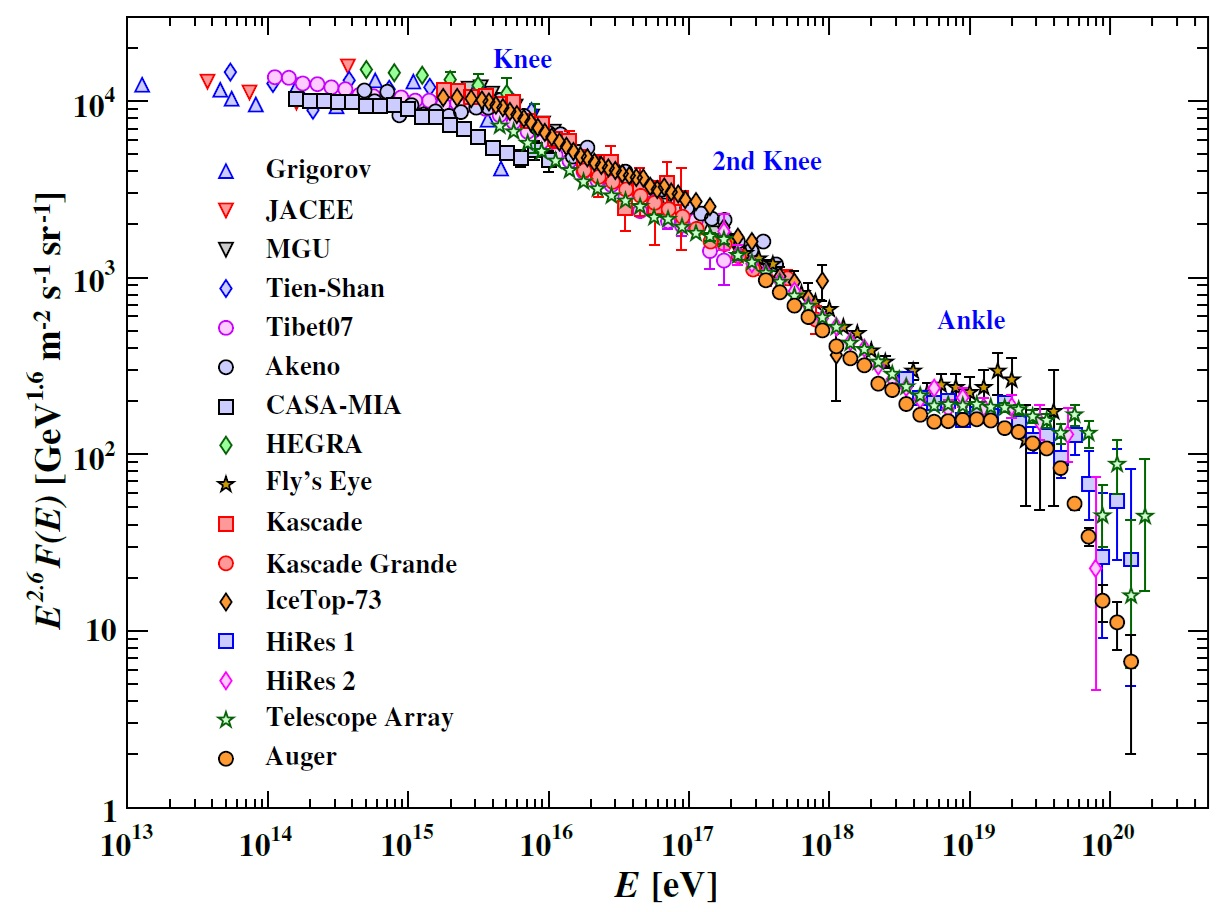
\includegraphics[width=\textwidth]{espectro_completo.jpg}
  \end{columns}
\end{frame}

\begin{frame}{Espectro de energía}
  \begin{columns}[c]
    \column{0.38\textwidth}
      \begin{itemize}
        \item El espectro de energía $J(E)\propto E^{-\gamma}$, con estructuras
          finas: \emph{rodilla} ($\sim3\times10^{15}$~eV), \emph{segunda
          rodilla} ($\sim10^{17}$~eV), \emph{tobillo} ($\sim5\times10^{18}$~eV).
        \item Supresión de flujo por encima de $4\times10^{19}$~eV, confirmada
          por Auger con alta significancia estadística.
        \item Pero el \textbf{espectro no dice de qué está hecho} el rayo cósmico.
      \end{itemize}
    \column{0.58\textwidth}
      \centering
      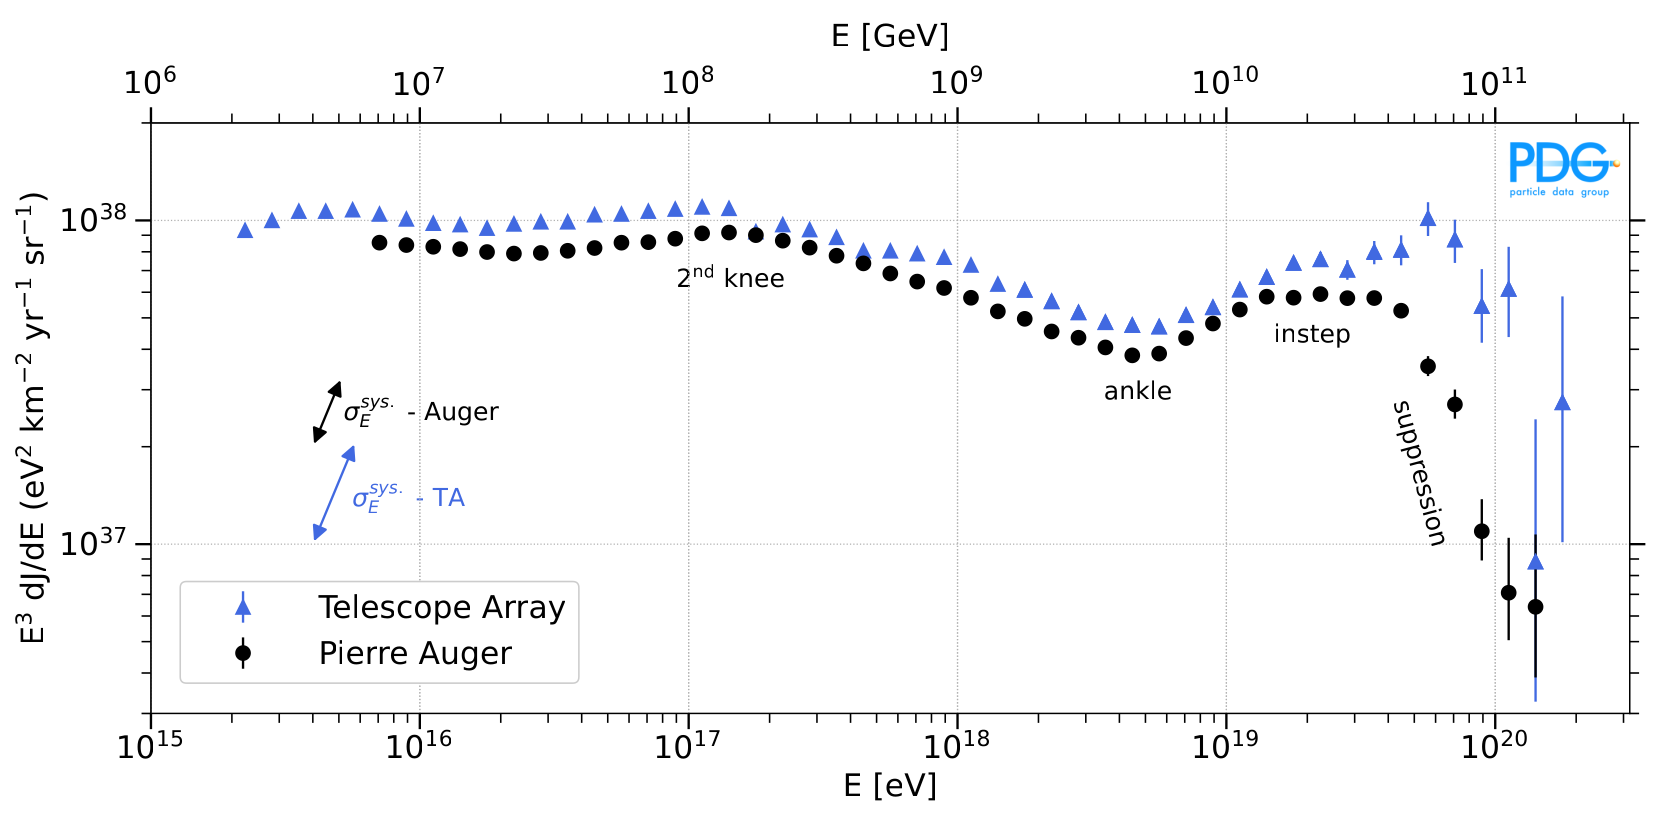
\includegraphics[width=\textwidth]{espectro_uhecr.png}
  \end{columns}
\end{frame}

\begin{frame}{El problema abierto: composición de masa}
  \begin{columns}[T]
    \column{0.44\textwidth}
      \begin{itemize}
        \item Un rayo cósmico primario inicia una \textbf{cascada hadrónica} en la
          alta atmósfera: una Lluvia Atmosférica Extensa (EAS).
        \item Un observable de composición central: $X_{\max}$, la profundidad
          atmosférica del máximo desarrollo de la cascada.
        \item Núcleos pesados (Fe) interactúan más alto $\Rightarrow$ $X_{\max}$
          \textbf{más superficial} que un protón de igual energía.
        \item Auger mide $X_{\max}$ con el FD --- pero \textbf{sólo
          $\sim$15\%} del tiempo (noches oscuras y despejadas).
      \end{itemize}
    \column{0.52\textwidth}
      \centering
      \vspace{0.6em}
      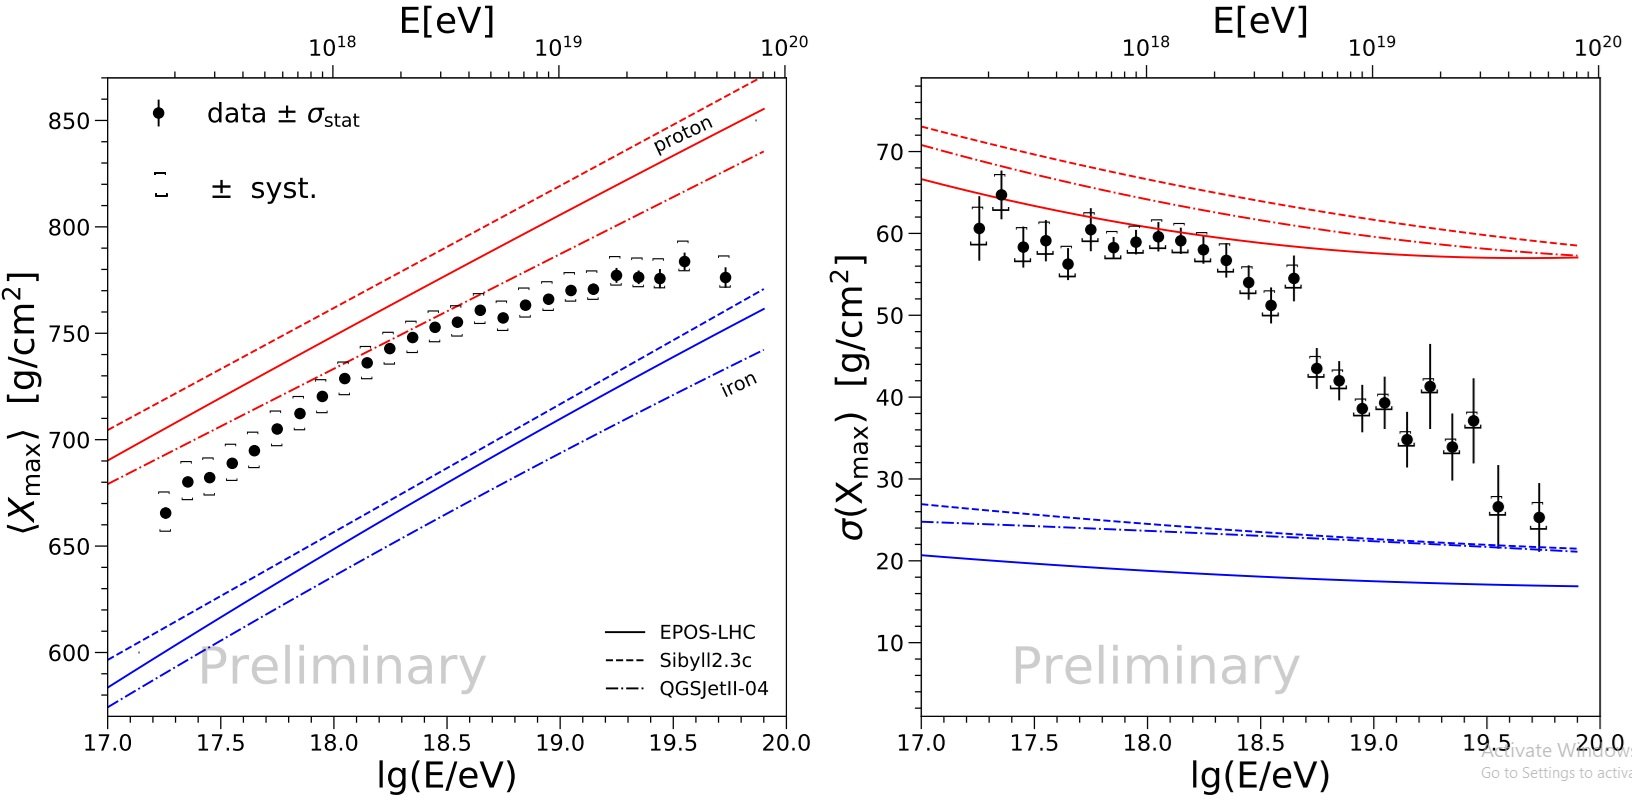
\includegraphics[width=\textwidth,height=4.4cm,keepaspectratio]{x_max.jpg}
  \end{columns}
\end{frame}

\begin{frame}{Anatomía de una lluvia: dos componentes muy distintas}
  \begin{columns}[T]
    \column{0.44\textwidth}
      \begin{itemize}
        \item \textbf{Componente electromagnética} ($e^\pm,\gamma$): numerosísima,
          se regenera y absorbe rápido (\emph{bremsstrahlung}, creación de pares).
        \item \textbf{Componente muónica}: producida en el decaimiento de piones y
          kaones, viaja casi en línea recta y penetra el suelo con poca pérdida
          de energía.
        \item Los detectores de superficie estándar \textbf{miden la suma de ambas}
          --- mezclando dos físicas distintas en una sola señal.
      \end{itemize}
    \column{0.52\textwidth}
      \centering
      \vspace{0.6em}
      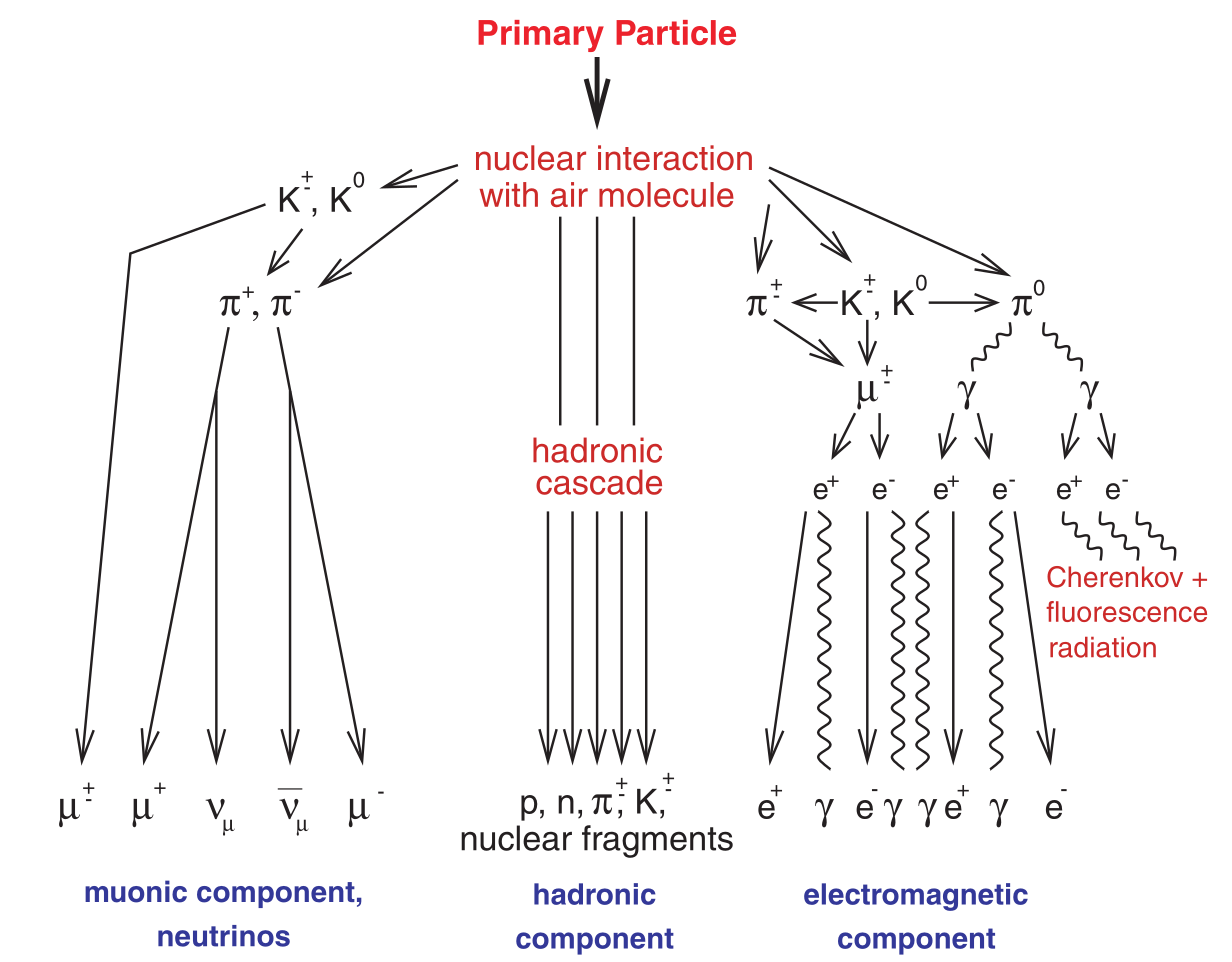
\includegraphics[width=\textwidth,height=4.4cm,keepaspectratio]{eas.png}
  \end{columns}
\end{frame}

% ============================================================
\section{El Observatorio Pierre Auger}

\begin{frame}{El Observatorio Pierre Auger}
  \begin{columns}[T]
    \column{0.5\textwidth}
      \begin{itemize}
        \item Mendoza, Argentina. \textbf{3000~km$^2$}, el detector de rayos
          cósmicos más grande del mundo.
        \item \textbf{Detección híbrida}: 1660 tanques Cherenkov en agua (SD,
          espaciado 1500~m) + 24 telescopios de fluorescencia (FD) en 4 sitios.
        \item El SD mide todo el año (duty cycle $\sim$100\%); el FD sólo de
          noche, calibra la escala de energía.
      \end{itemize}
    \column{0.48\textwidth}
      \centering
      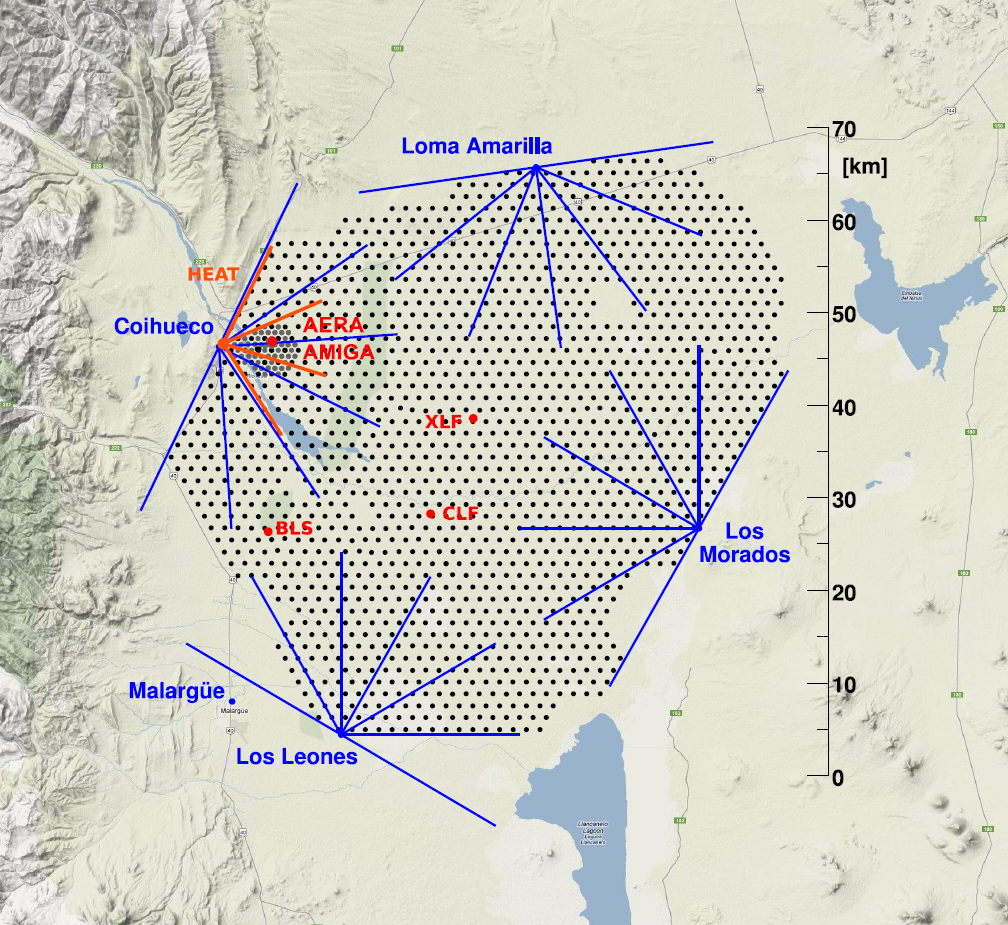
\includegraphics[width=\textwidth,height=5.3cm,keepaspectratio]{mapa_auger.png}
  \end{columns}
\end{frame}

\begin{frame}{AugerPrime}
  \begin{columns}[c]
    \column{0.44\textwidth}
      \begin{itemize}
        \item La gran actualización del Observatorio, ya desplegada.
        \item Un \textbf{Centellador de Superficie} (SSD, $3.8$~m$^2$) sobre cada
          tanque Cherenkov: responde distinto a fotones/electrones que a muones.
        \item La combinación WCD+SSD permite \emph{desenredar estadísticamente}
          las dos componentes en superficie --- pero no las separa físicamente.
      \end{itemize}
    \column{0.5\textwidth}
      \centering
      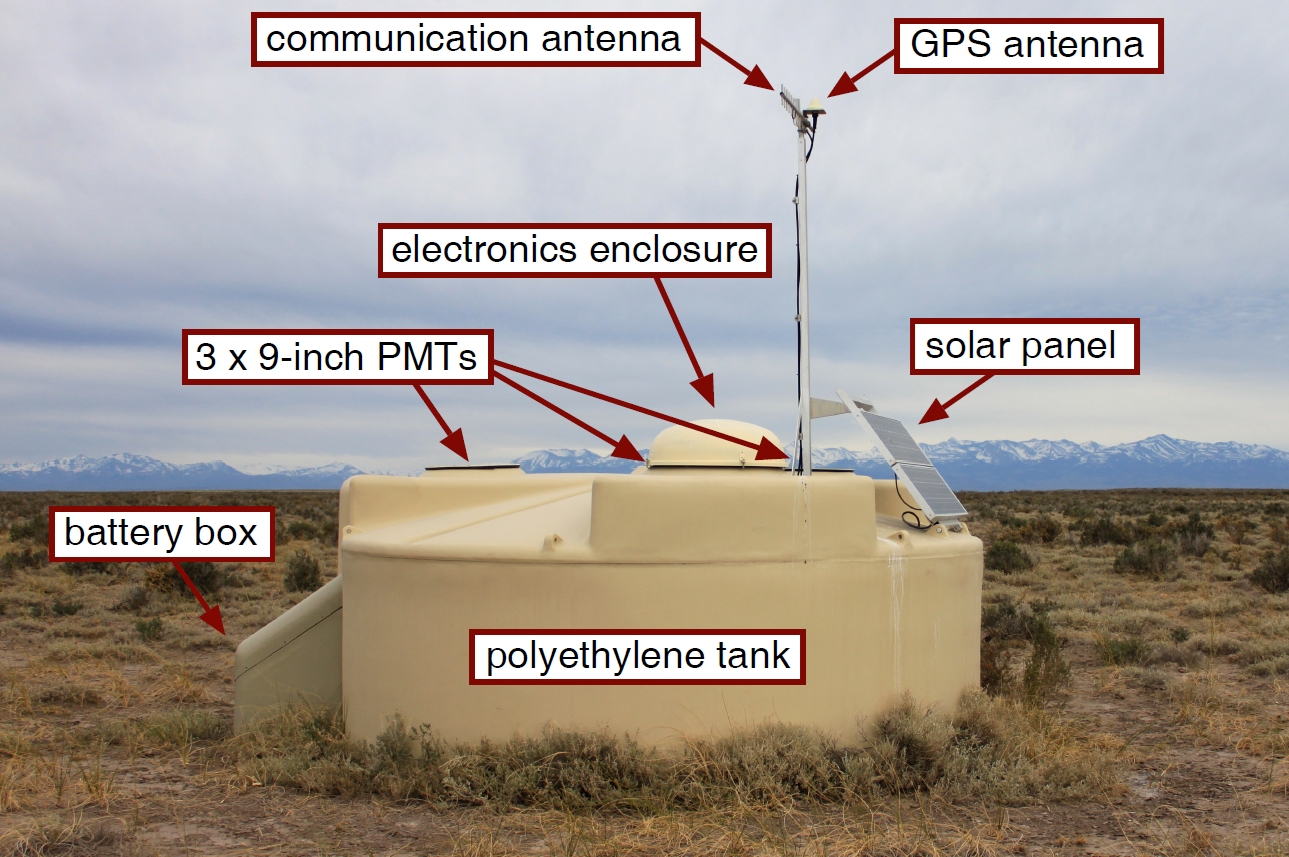
\includegraphics[width=\textwidth,height=5.1cm,keepaspectratio]{ssd.png}
  \end{columns}
\end{frame}

\begin{frame}{AMIGA y el Detector Subterráneo de Muones (UMD)}
  \begin{columns}[T]
    \column{0.48\textwidth}
      \begin{itemize}
        \item \textbf{Enterrado 2.3~m} junto a cada tanque de superficie
          $\Rightarrow \sim$\textbf{540~g/cm$^2$} de tierra --- el equivalente
          a una atmósfera terrestre completa adicional.
        \item 3 módulos centelladores de 10~m$^2$ c/u, 64 tiras por módulo,
          lectura con fotomultiplicadores de silicio (SiPM).
        \item Parte de la extensión \emph{Infill} (750~m) del arreglo, apuntando
          a la transición galáctico/extragaláctico ($\sim10^{17}$~eV).
      \end{itemize}
    \column{0.48\textwidth}
      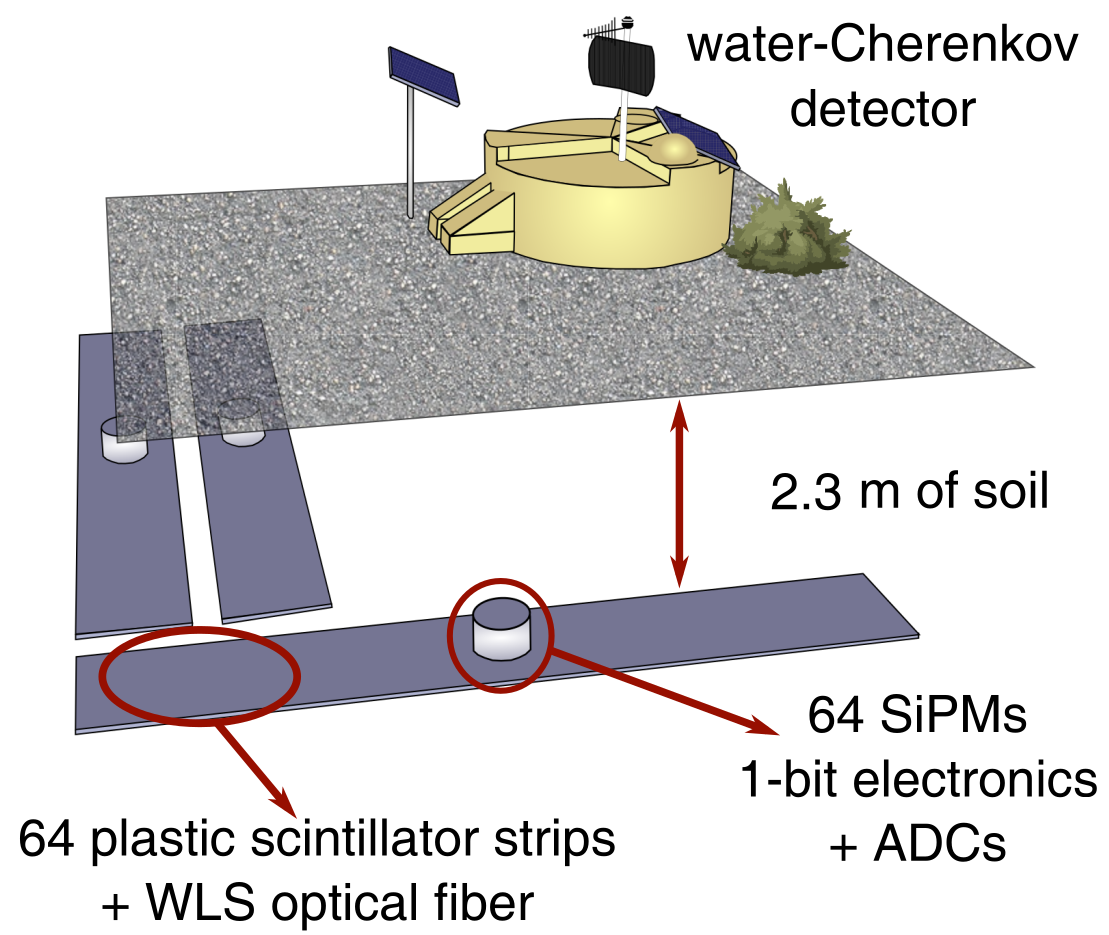
\includegraphics[width=\textwidth]{umd.png}
  \end{columns}
\end{frame}

\begin{frame}{¿Por qué el UMD es un detector distinto?}
  \begin{block}{El blindaje de tierra actúa como \textbf{doble filtro}}
    \begin{enumerate}
      \item \textbf{Absorción electromagnética total}: 2.3~m de tierra extinguen
        por completo $e^\pm/\gamma$. La señal del UMD es un frente
        \alert{muónico puro} --- sin la convolución $S_{EM}+S_\mu$ del SD.
      \item \textbf{Umbral cinemático}: sólo atraviesan la tierra los muones
        que llegan al \textbf{nivel del suelo} con $E_\mu \gtrsim 1$~GeV$/\cos\theta$
        (antes de cruzar los 2.3~m). El UMD selecciona así la población de
        muones de \emph{alta energía}, nacidos en las primeras generaciones
        hadrónicas.
    \end{enumerate}
  \end{block}
  \vspace{0.5em}
  \centering
  \Large Esta es la idea central del trabajo: usar el UMD para aislar\\
  la física de la componente muónica pura.
\end{frame}

% ============================================================
\section{Fenomenología: el origen de la asimetría azimutal}

\begin{frame}{El plano de la lluvia y la ruptura de simetría}
  \begin{columns}[T]
    \column{0.46\textwidth}
      \begin{itemize}
        \item Lluvia vertical ($\theta_{sh}=0^\circ$): simetría circular perfecta
          --- todos los detectores a igual $r$ ven la misma densidad.
        \item Lluvia inclinada ($\theta_{sh}>0^\circ$): el plano de la lluvia ya
          no es paralelo al suelo.
        \item Aparecen dos regiones privilegiadas:
        \begin{itemize}
          \item \textbf{Temprana} ($\phi\approx0^\circ$): golpea el suelo primero,
            recorrió \emph{menos} atmósfera.
          \item \textbf{Tardía} ($\phi\approx\pm180^\circ$): golpea después,
            recorrió \emph{más} atmósfera.
        \end{itemize}
      \end{itemize}
    \column{0.5\textwidth}
      \centering
      \vspace{0.6em}
      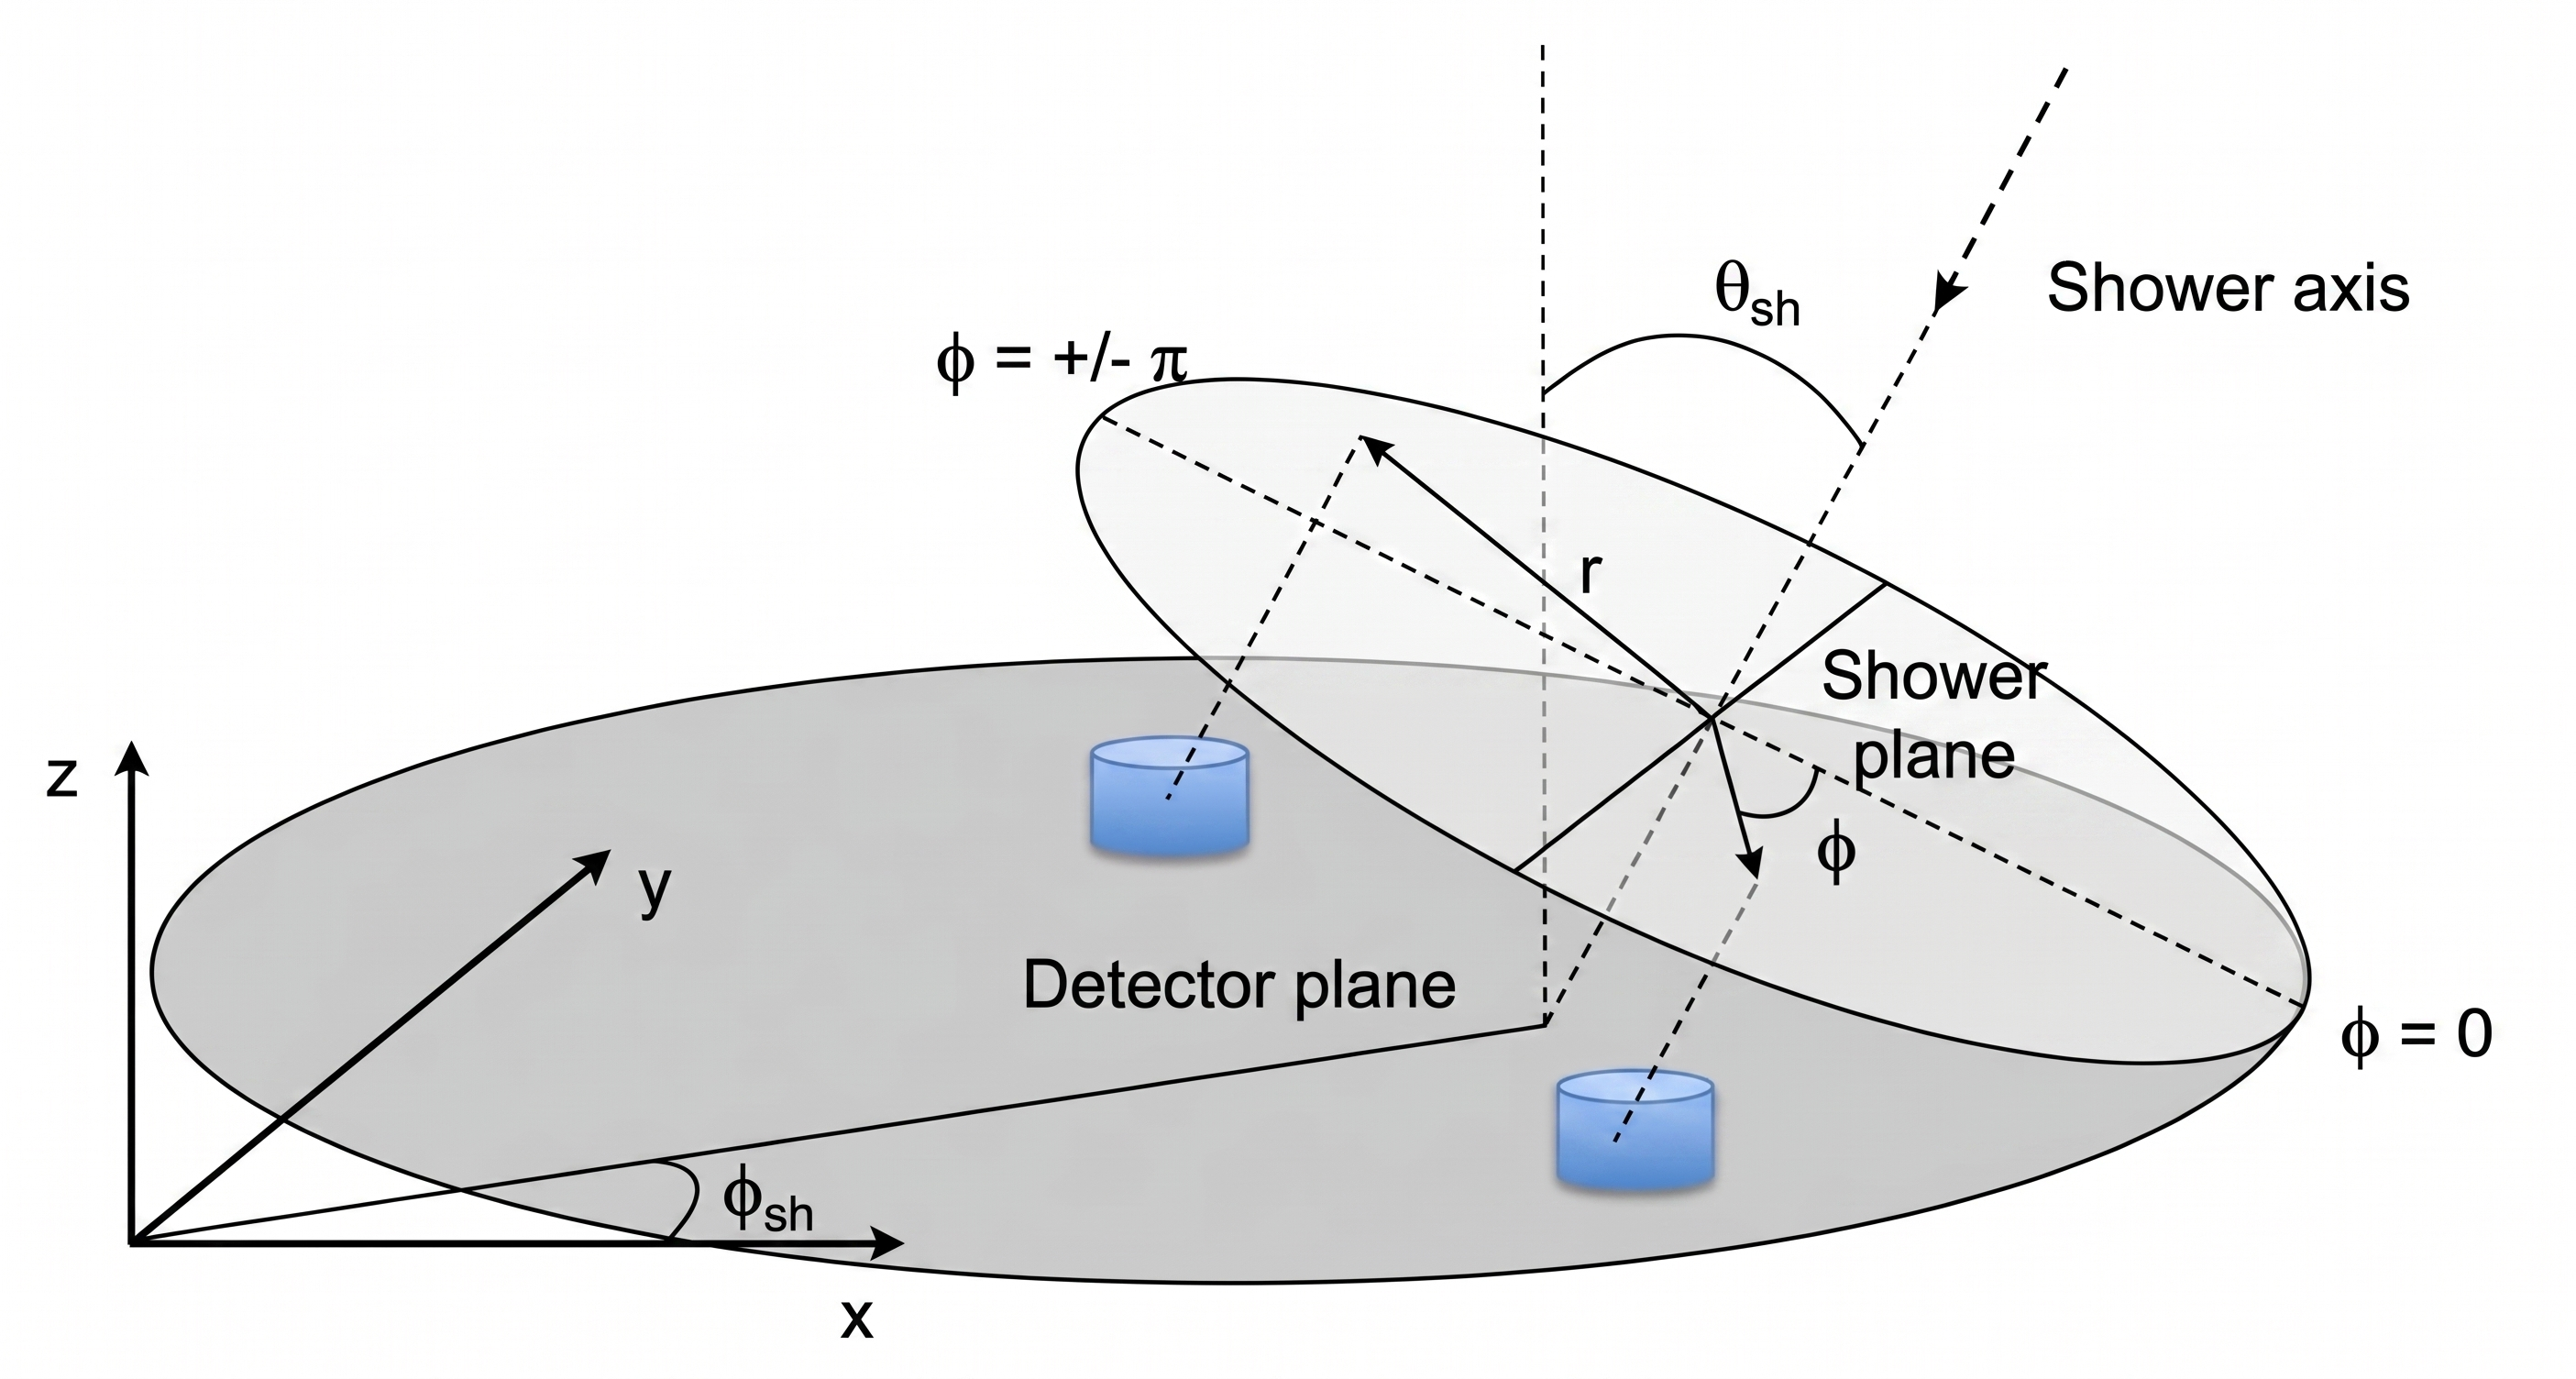
\includegraphics[width=\textwidth,height=4.2cm,keepaspectratio]{esquema_lluvia.jpeg}
  \end{columns}
\end{frame}

\begin{frame}{Mecanismo 1: atenuación atmosférica}
  \begin{itemize}
    \item La región tardía atraviesa \textbf{más atmósfera} antes de llegar al
      suelo $\Rightarrow$ la cascada se absorbe más en su camino.
    \item Resultado: un \alert{exceso de densidad en la región temprana}.
    \item Actúa sobre ambas componentes, pero con mayor magnitud sobre la EM (longitud
      de radiación corta) que sobre los muones (ionización, mucho más penetrantes).
  \end{itemize}
  \begin{block}{Signo}
    Atenuación atmosférica $\Rightarrow A_1 > 0$
  \end{block}
\end{frame}

\begin{frame}{Mecanismo 2: proyección geométrica del disco}
  \begin{columns}[T]
    \column{0.52\textwidth}
      \begin{itemize}
        \item La lluvia está inclinada: para llegar al mismo $r$, el frente
          de muones incide sobre el suelo con un \textbf{ángulo distinto} en
          la región temprana que en la tardía
          ($\theta_{\text{early}}\neq\theta_{\text{late}}$).
        \item Esa diferencia cambia el área efectiva de cada estación ---
          un efecto \textbf{puramente geométrico de proyección}.
        \item Bertou \& Billoir (GAP-2000-017) cuantifican este término
          $\mathcal{A}_{geo}$.
      \end{itemize}
    \column{0.44\textwidth}
      \centering
      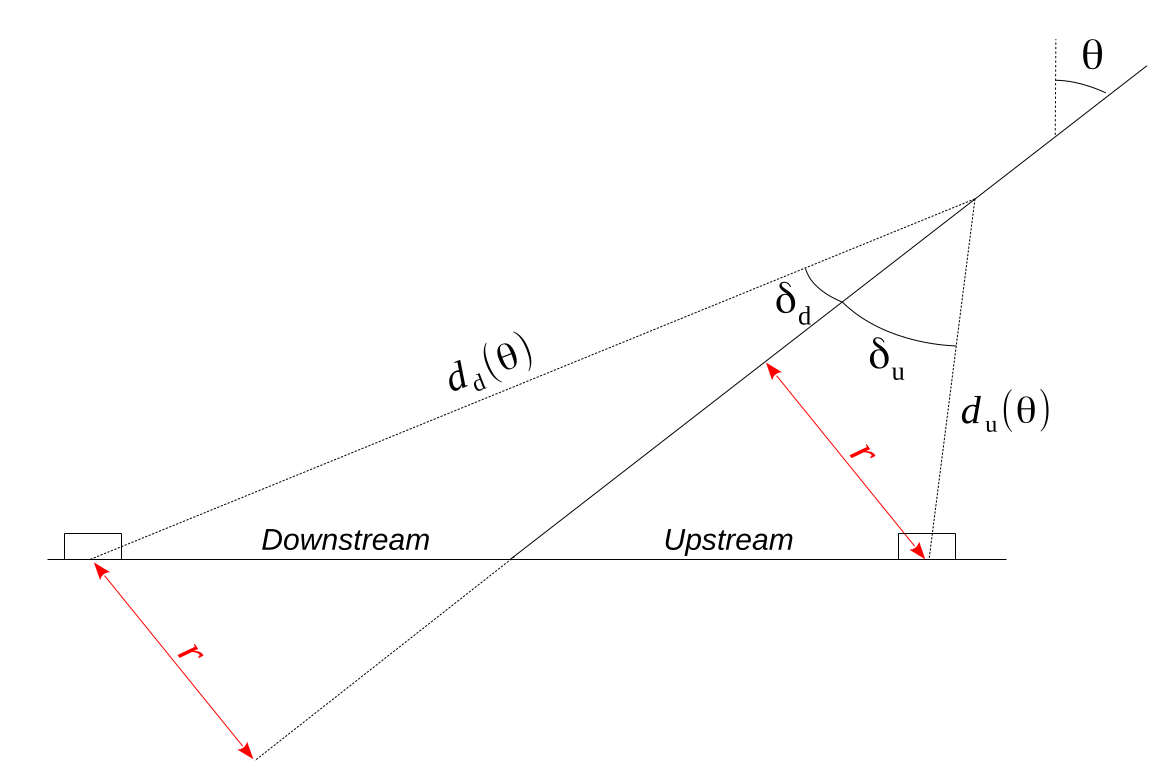
\includegraphics[width=\textwidth,height=3.7cm,keepaspectratio]{efecto_geo.png}
  \end{columns}
  \begin{block}{Signo}
    \small Para un plano ideal, la proyección geométrica \textbf{también} da
    $A_1 > 0$ (GAP-2026-041, \S2.2).
  \end{block}
\end{frame}

\begin{frame}{Mecanismo 3: divergencia cinemática (Cazón \textit{et al.})}
  \badgeMATH
  \begin{columns}[T]
    \column{0.52\textwidth}
      \begin{itemize}\small
        \item Distinto de la proyección de Billoir: aquí importa la
          \textbf{distancia finita} $D$ entre producción y suelo.
        \item El muón nace del decaimiento $\pi/K$ con momento transverso
          $p_t$ $\Rightarrow$ ángulo de apertura $\sin\alpha\simeq cp_t/E$.
        \item Espectro angular de emisión (\emph{ADF} de Cazón):
          $$\frac{dN}{d\Omega}(\alpha) \propto \cos\alpha\,
          \exp\!\left(-\frac{E\sin\alpha}{cQ}\right)$$
        \item Densidad en el suelo: $S(d,\alpha)\propto d^{-2}\,dN/d\Omega$.
      \end{itemize}
    \column{0.44\textwidth}
      \centering
      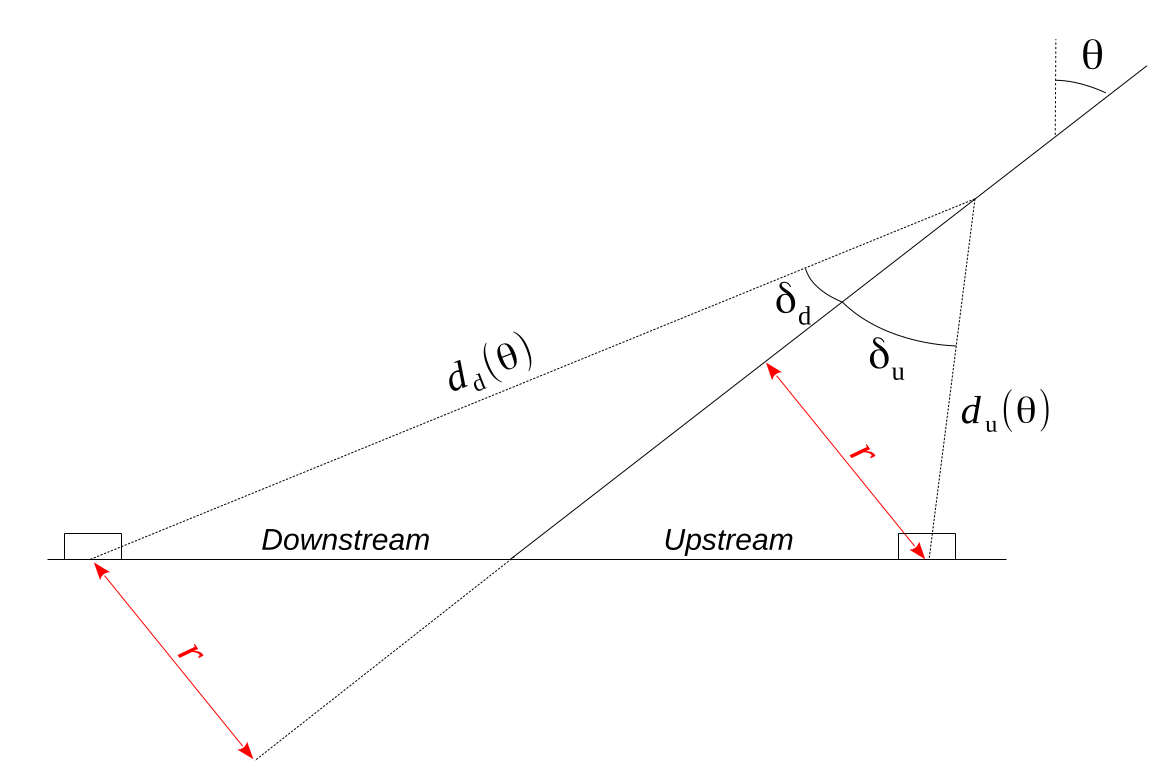
\includegraphics[width=\textwidth,height=3.7cm,keepaspectratio]{efecto_geo.png}
  \end{columns}
\end{frame}

\begin{frame}{¿Positivo o negativo? La energía de cruce}
  \badgeMATH
  \begin{equation*}
    \frac{S_{\text{tardío}}}{S_{\text{temprano}}} \approx
    \underbrace{\left(\frac{d_{\text{temprano}}}{d_{\text{tardío}}}\right)^{\!2}}_{\text{espacial}\,<\,1}
    \cdot
    \underbrace{\frac{\cos\alpha_{\text{tardío}}}{\cos\alpha_{\text{temprano}}}}_{\text{esp.\ de fases}\,>\,1}
    \cdot
    \underbrace{\exp\!\left(\frac{(\sin\alpha_{\text{temprano}}-\sin\alpha_{\text{tardío}})E}{cQ}\right)}_{\text{ganancia cinemática}\,>\,1}
  \end{equation*}
  \begin{itemize}\small
    \item Sólo el tercer factor depende de $E$, y es
      \textbf{monótonamente creciente}: $\approx1$ (sin efecto) a baja
      $E$, relevante recién a alta $E$ --- existe una \textbf{energía de
      cruce $E^*$} por debajo de la cual domina el término espacial
      (favorece la región temprana, $A_1>0$).
    \item Población B (baja $E$) contribuye entonces con el
      \textbf{mismo signo} que la atenuación --- no con el opuesto.
    \item En $r{=}1200$~m, $\theta{=}35^\circ$ ($D{=}7.5$~km,
      $Q{=}0.2$~GeV, $\gamma{=}2.6$): $A_1\simeq+0.16$ en el umbral
      tipo SD, $+0.02$ en el umbral del UMD, negativo recién por
      encima de $\sim2$~GeV.
  \end{itemize}
  \vspace{0.2em}
  \centering
  \alert{Mecanismo real y positivo en casi todo el rango relevante ---
  pero predice el UMD \emph{menos} positivo que el SD: no explica por
  sí solo el contraste observado.}
\end{frame}

\begin{frame}{El observable: el primer armónico azimutal}
  \begin{equation*}
    S(r,\phi,\theta) = \langle S(r,\theta) \rangle \big(1 + A_1(r,\theta)\cos\phi\big)
  \end{equation*}
  \begin{itemize}
    \item $A_1 > 0$: exceso temprano; $A_1 < 0$: exceso tardío --- requiere
      un mecanismo \emph{adicional} a los dos ya vistos.
    \item Fase fijada en $\phi_0=0$ (línea temprano-tardía), siguiendo la
      convención de estudios previos con el SD.
    \item Deflexión geomagnética: efecto de segundo orden aquí; dominante
      sólo en lluvias muy horizontales ($\theta>80^\circ$).
  \end{itemize}
  \vspace{0.2em}
  \centering
  \alert{Si los dos mecanismos conocidos dan siempre $A_1>0$,
  ¿qué pasa si medimos $A_1<0$?}
\end{frame}

% ============================================================
\section{Método: simulaciones y reconstrucción}

\begin{frame}{De CORSIKA a un valor de $A_1$}
  \begin{center}
  \begin{tikzpicture}[node distance=0.55cm, every node/.style={font=\small}]
    \node[draw, rounded corners, fill=itedaTeal, text=white, minimum width=2.6cm, minimum height=0.9cm] (c) {CORSIKA};
    \node[draw, rounded corners, fill=itedaTeal, text=white, minimum width=2.6cm, minimum height=0.9cm, right=of c] (o) {Offline};
    \node[draw, rounded corners, fill=itedaOrange, text=white, minimum width=2.9cm, minimum height=0.9cm, right=of o] (a) {ajuste $A_1(r,\theta)$};
    \draw[-{Latex}] (c) -- (o);
    \draw[-{Latex}] (o) -- (a);
  \end{tikzpicture}
  \end{center}
  \begin{itemize}
    \item Producción \texttt{icrc2025-test7}: p / He / O / Fe, SIBYLL~2.3e (+QGSJET-III,
      EPOS-LHC-R), $\log_{10}(E/\text{eV})\in[17.5,18.0]$, $\theta\in[0^\circ,65^\circ]$.
    \item Dos topologías de evaluación:
    \begin{itemize}
      \item \textbf{Anillo Denso}: 12 estaciones virtuales a $r=450$~m fijo,
        cada $30^\circ$ --- entorno de control.
      \item \textbf{Infill}: arreglo real de 750~m, espectro continuo de $r$.
    \end{itemize}
  \end{itemize}
\end{frame}

\begin{frame}{Validación: la reconstrucción es fiable}
  \begin{columns}[T]
    \column{0.5\textwidth}
      \centering
      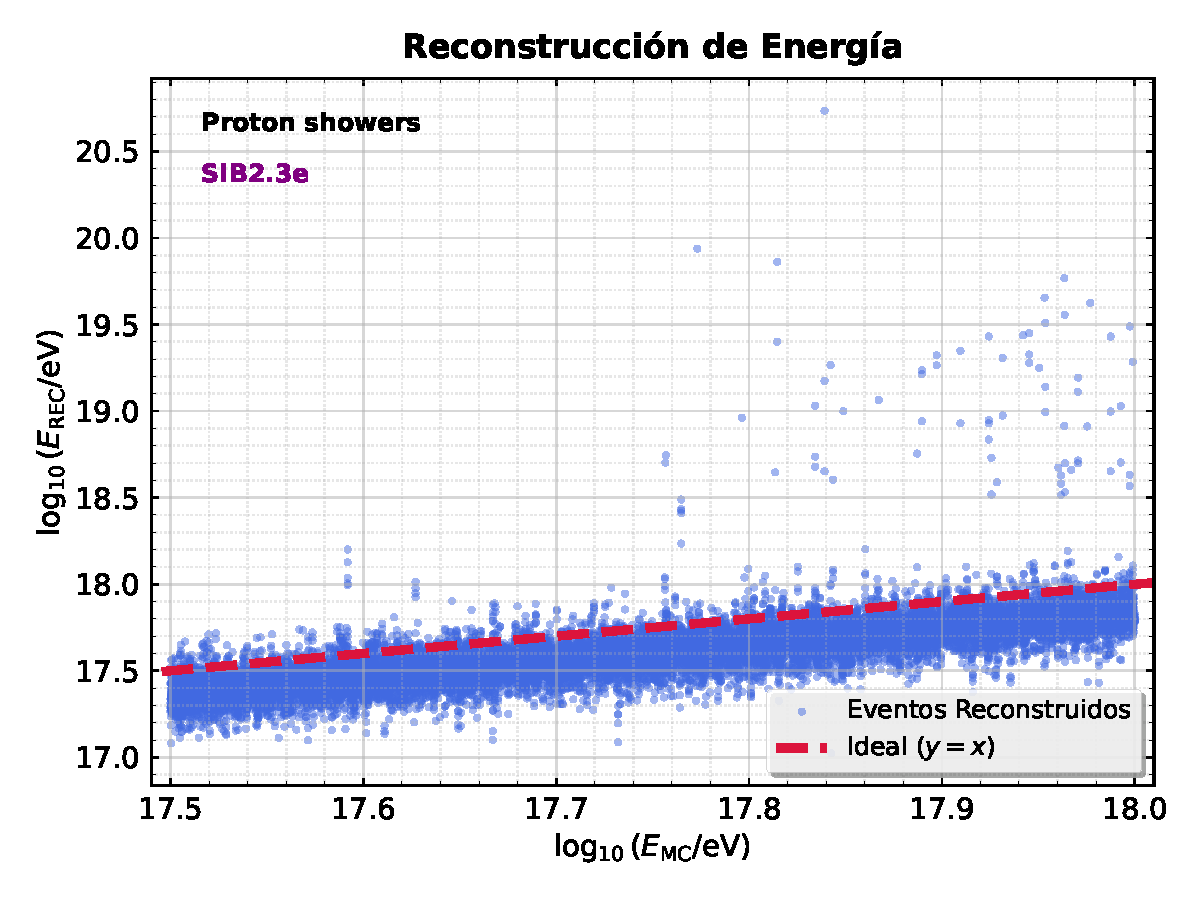
\includegraphics[width=\textwidth,height=4.6cm,keepaspectratio]{energy_reconstr.pdf}
    \column{0.5\textwidth}
      \centering
      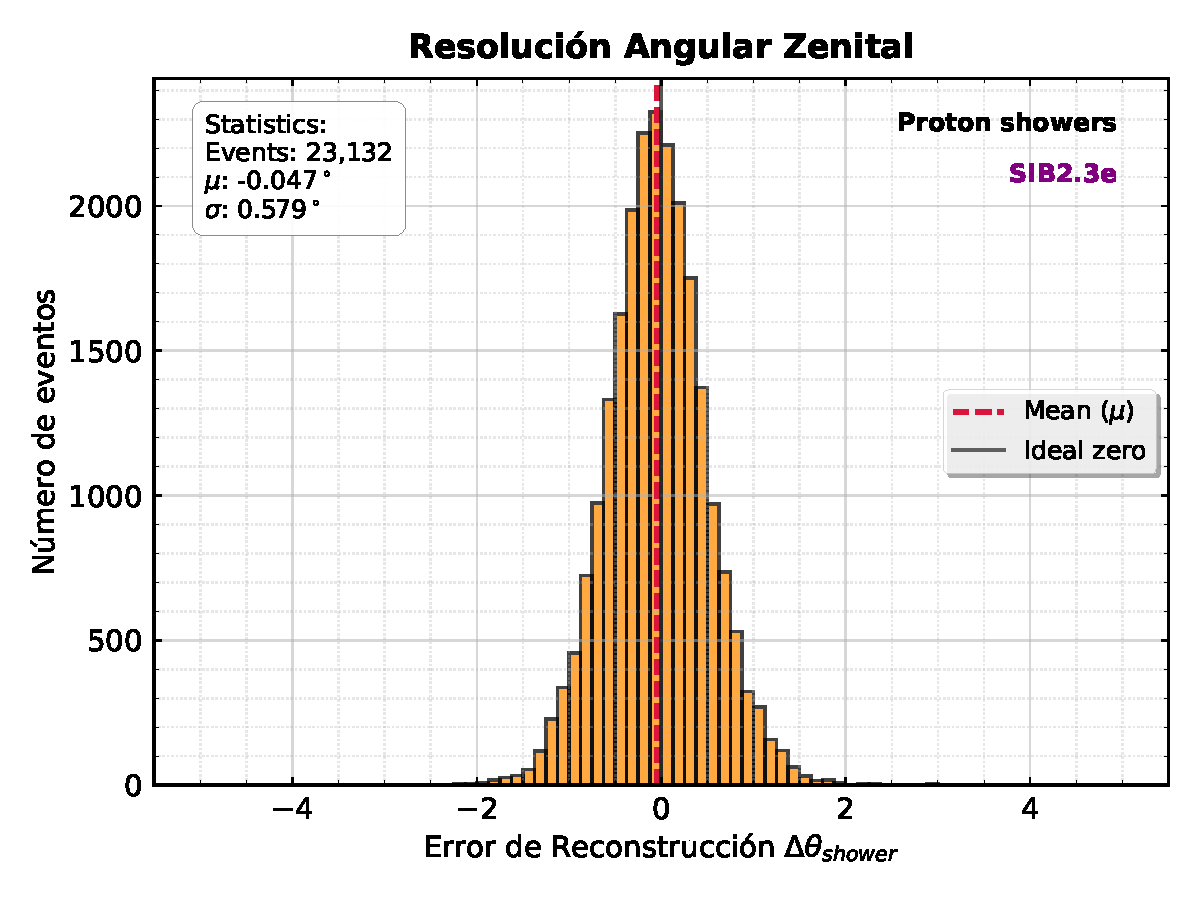
\includegraphics[width=\textwidth,height=4.6cm,keepaspectratio]{theta_bias.pdf}
  \end{columns}
  \begin{itemize}
    \item Energía: subestimación sistemática $\mu\approx-0.14$ en $\Delta\log_{10}E$
      (\emph{muon deficit} de los modelos hadrónicos), $\sigma\approx0.11$.
    \item Ángulo cenital $\theta$: sesgo $<0.05^\circ$, resolución
      $\sigma\approx0.6^\circ$ --- no introduce modulación espuria en $A_1$.
    \item Ángulo azimutal $\phi$: igual de sólido (sesgo $\approx-0.005^\circ$,
      $\sigma\approx2.2^\circ$).
  \end{itemize}
\end{frame}

% ============================================================
\section{Resultados I: el Anillo Denso}

\begin{frame}{El Anillo Denso: un ejemplo de ajuste}
  \badgeMC
  \begin{columns}[T]
    \column{0.5\textwidth}
      \centering
      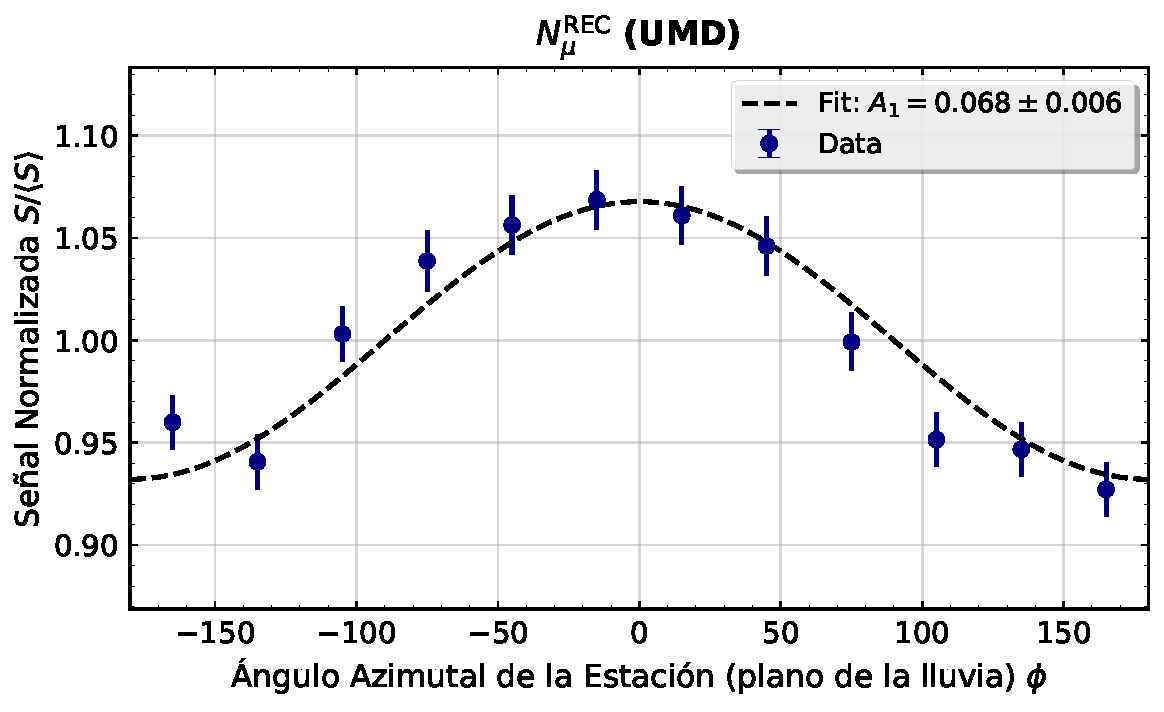
\includegraphics[width=\textwidth,height=5.2cm,keepaspectratio]{ajuste_umd_rec_bin9.pdf}
    \column{0.46\textwidth}
      \begin{itemize}
        \item 12 estaciones virtuales, $r=450$~m, bin más inclinado
          ($59^\circ$--$65^\circ$).
        \item Modulación clara: diferencia pico-a-pico
          \alert{$\approx14\%$} ($\pm7\%$ respecto a la media).
        \item El ajuste armónico de primer orden reproduce los datos con
          $\chi^2_\nu\approx1$.
      \end{itemize}
  \end{columns}
\end{frame}

\begin{frame}{$A_1$ vs.\ $\theta$: UMD y SD cruzan de dominancia}
  \badgeMC
  \begin{columns}[T]
    \column{0.55\textwidth}
      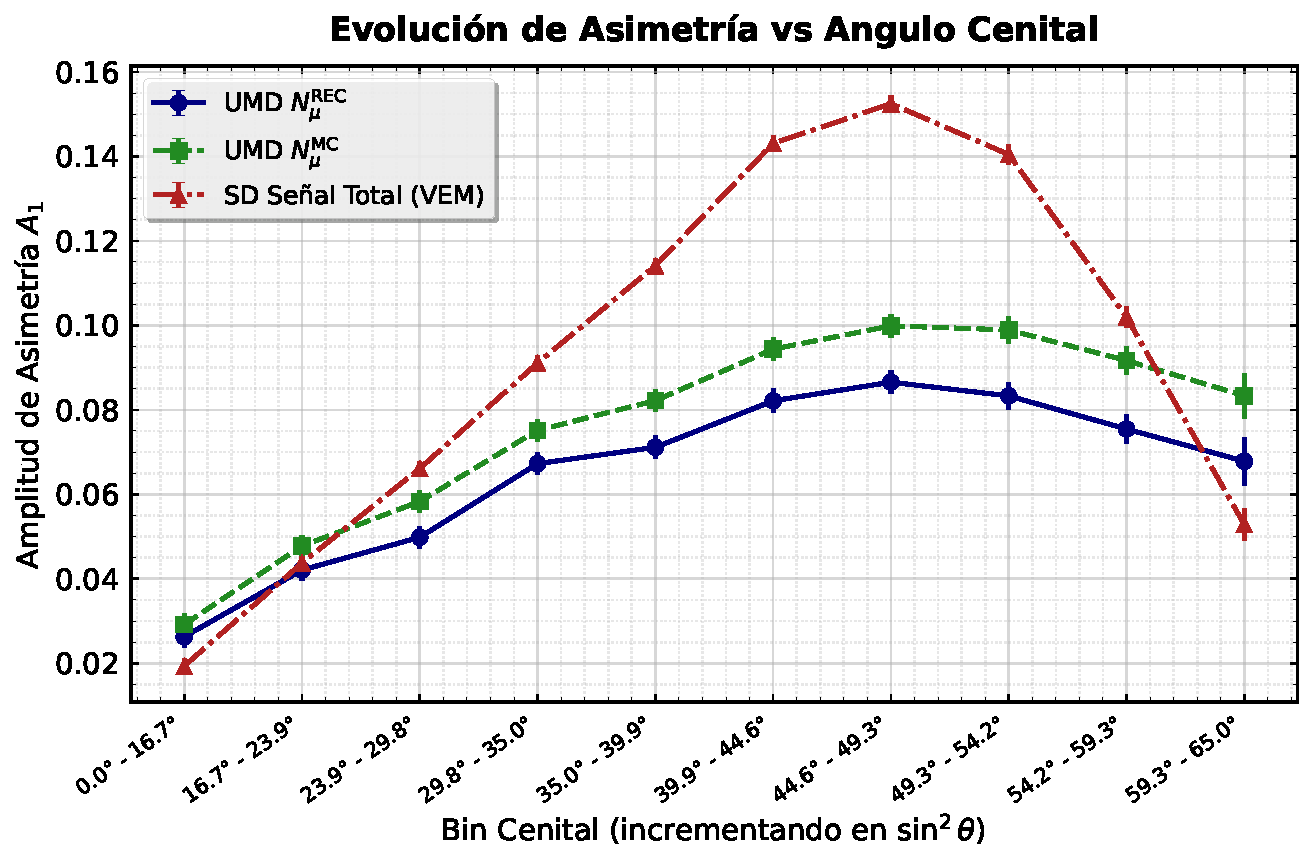
\includegraphics[width=\textwidth]{evolucion_asimetria_vs_theta.pdf}
    \column{0.4\textwidth}
      \begin{itemize}
        \item $\theta$ bajo: el SD (dominado por EM) tiene $A_1$ mucho mayor
          que el UMD.
        \item $\theta \gtrsim 50^\circ$: la componente EM se absorbe casi por
          completo --- el SD cae \textbf{por debajo} del UMD.
        \item El UMD crece de forma suave y estable, con una leve caída
          recién en los bines más inclinados.
      \end{itemize}
  \end{columns}
\end{frame}

\begin{frame}{Robustez del observable}
  \badgeMC
  \begin{columns}[T]
    \column{0.33\textwidth}
      \centering
      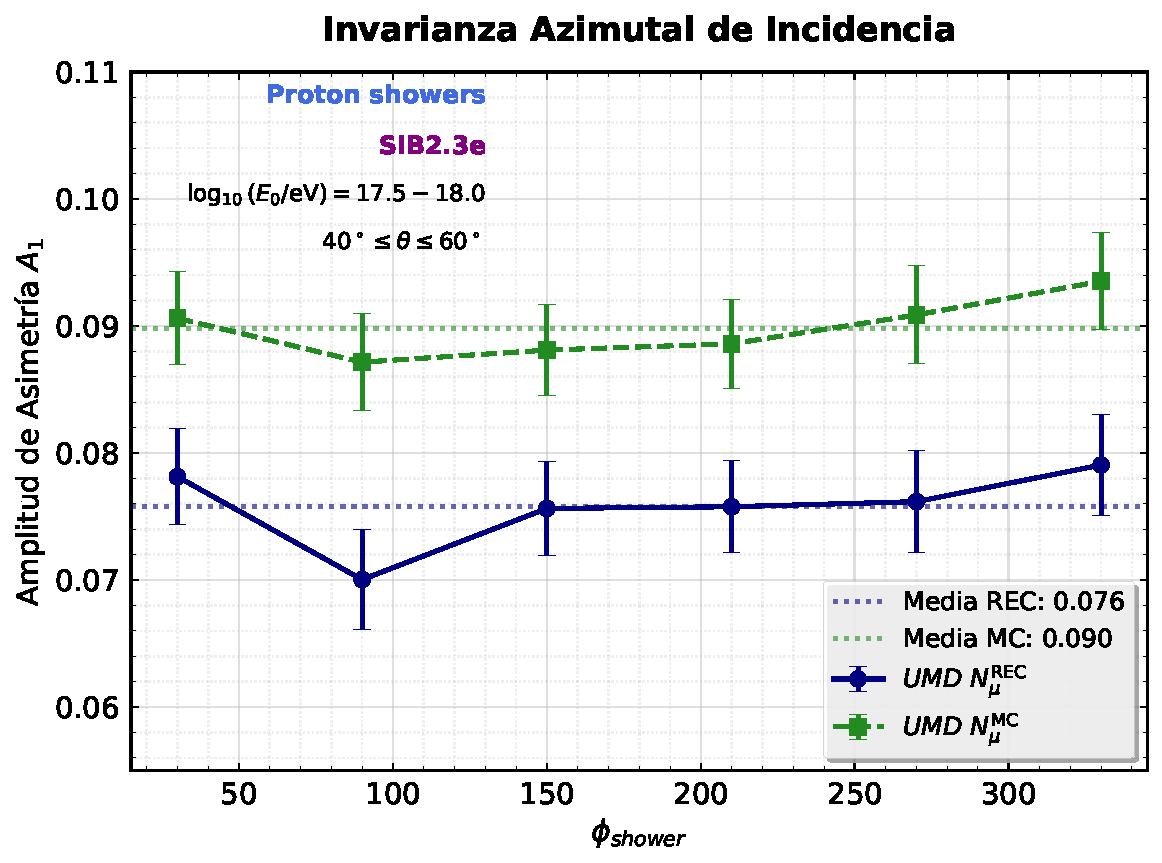
\includegraphics[width=\textwidth]{densering_sys_isotropy.pdf}
    \column{0.33\textwidth}
      \centering
      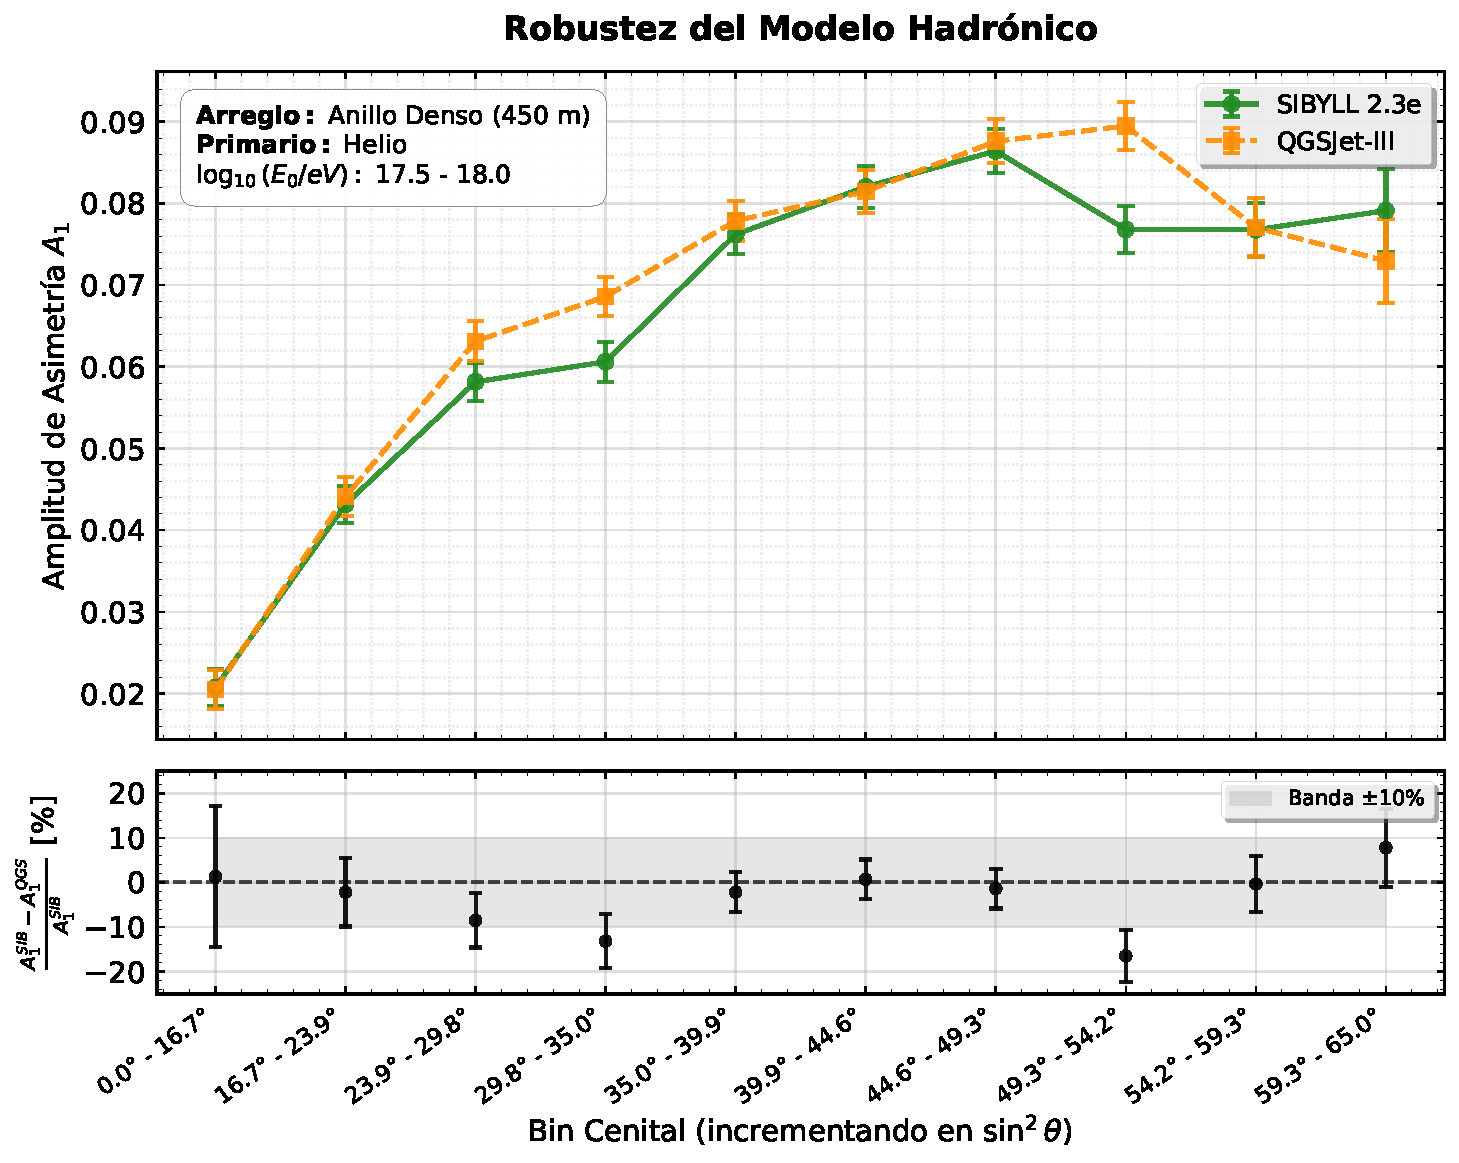
\includegraphics[width=\textwidth]{hadronic_uncertainty_helium.pdf}
    \column{0.33\textwidth}
      \centering
      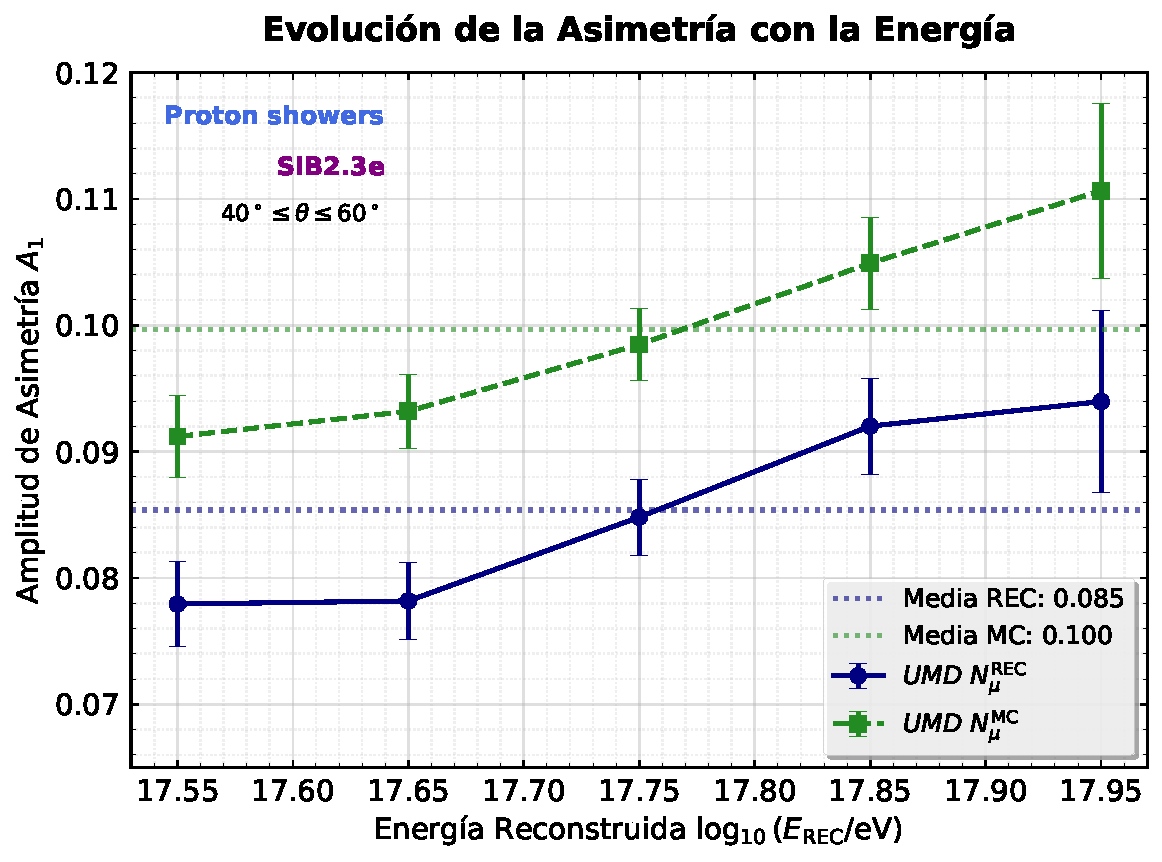
\includegraphics[width=\textwidth]{densering_sys_energy.pdf}
  \end{columns}
  \begin{itemize}
    \item $A_1$ es independiente de la dirección de arribo, y estable entre
      SIBYLL~2.3e y QGSJET-III (dentro de $\pm10\%$).
    \item Crece levemente con $E$ ($\Delta A_1\approx0.015$) --- posible
      indicio de su relación con $X_{\max}$, que se retoma más adelante.
  \end{itemize}
\end{frame}

\begin{frame}{Discriminación de masa: protón vs.\ hierro}
  \badgeMC
  \begin{columns}[c]
    \column{0.58\textwidth}
      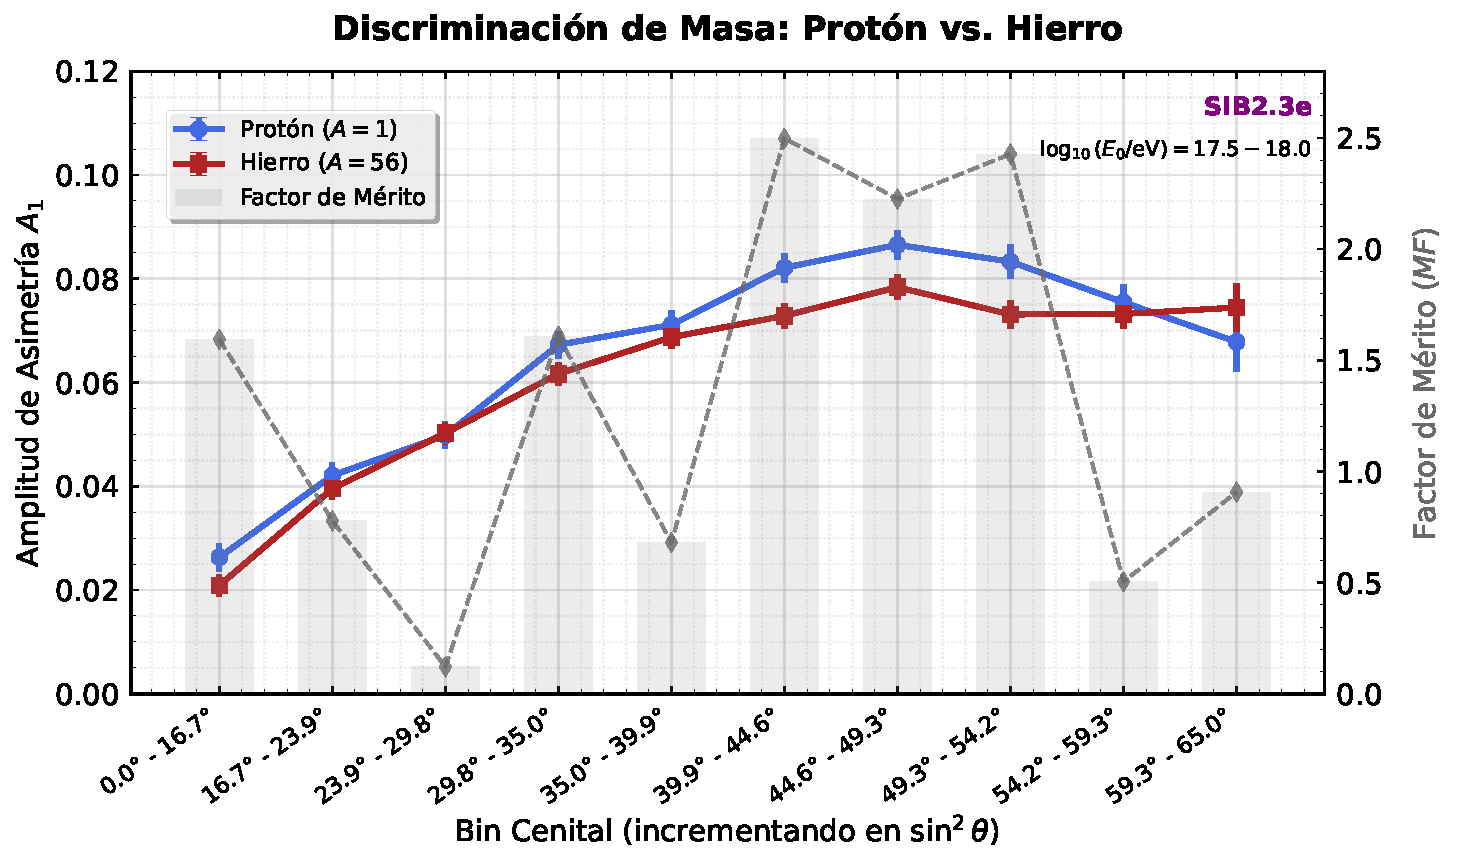
\includegraphics[width=\textwidth]{mass_discrimination_mf.pdf}
    \column{0.38\textwidth}
      \begin{itemize}
        \item $\langle A_1^{\text{p}}\rangle > \langle A_1^{\text{Fe}}\rangle$
          sistemáticamente.
        \item \emph{Hipótesis}: relacionada con un $X_{\max}$ más profundo
          en el protón.
      \end{itemize}
      \vspace{0.6em}
      \begin{equation*}
        MF=\dfrac{|\langle A_1^p\rangle-\langle A_1^{Fe}\rangle|}
        {\sqrt{\sigma_p^2+\sigma_{Fe}^2}}
      \end{equation*}
      \vspace{0.4em}
      \alert{\emph{Sweet spot}: $MF\approx2.5$ en $\theta=40^\circ$--$55^\circ$.}
  \end{columns}
\end{frame}

% ============================================================
\section{Resultados II: el arreglo \textit{Infill} y la inversión del SD}

\begin{frame}{El UMD en el arreglo real: $A_1(r,\theta)$}
  \badgeMC
  \begin{columns}[c]
    \column{0.62\textwidth}
      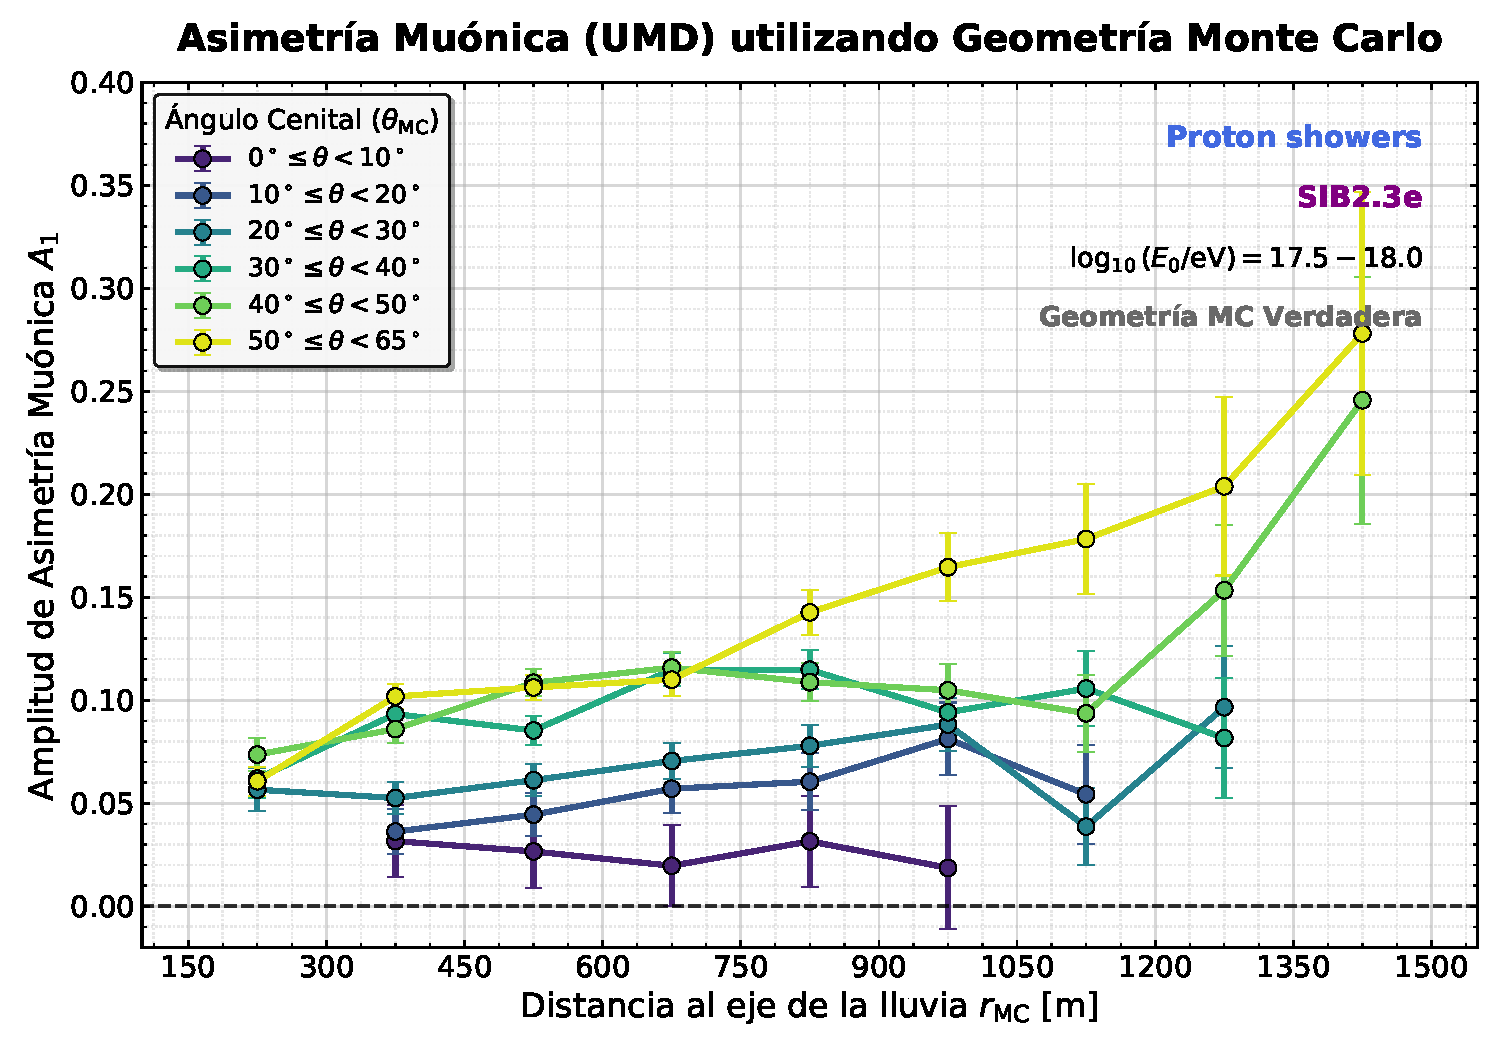
\includegraphics[width=\textwidth]{global_a1_vs_r_theta_mc.pdf}
    \column{0.34\textwidth}
      \begin{itemize}
        \item Régimen vertical ($\theta<10^\circ$): $A_1\approx0$.
        \item Régimen intermedio: crecimiento con saturación/meseta.
        \item Régimen inclinado ($\theta\gtrsim40^\circ$): crecimiento
          monótono, sin saturación, robusto hasta 1500~m.
      \end{itemize}
  \end{columns}
\end{frame}

\begin{frame}{El hallazgo central: la inversión de signo del SD}
  \badgeMC
  \begin{columns}[c]
    \column{0.62\textwidth}
      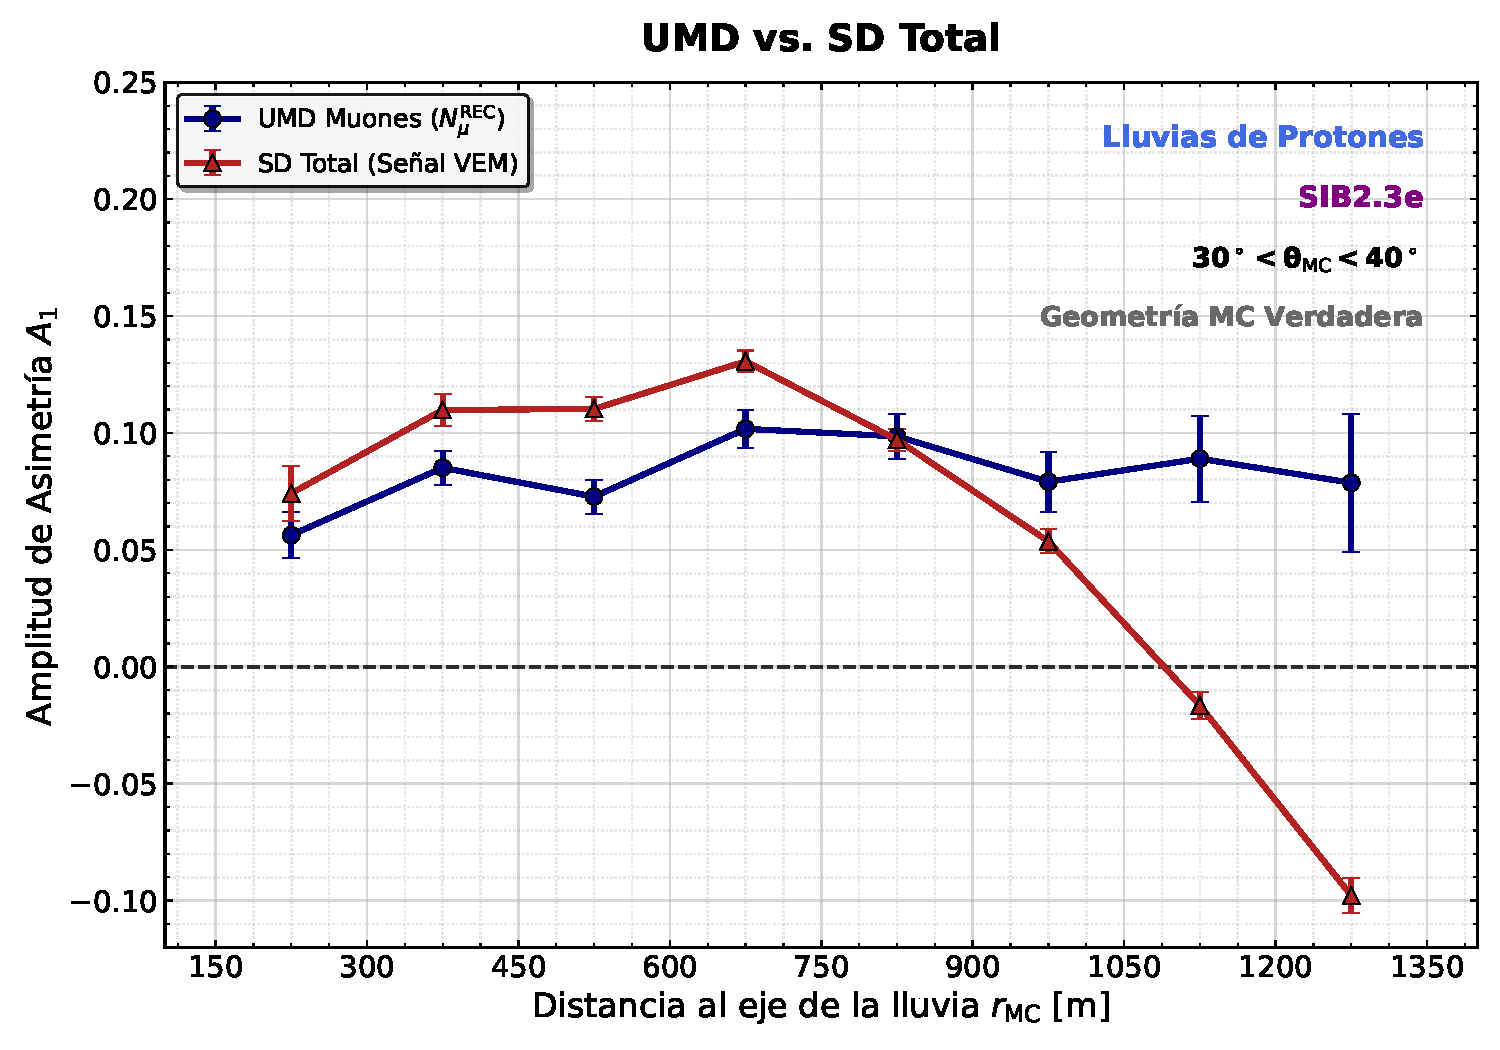
\includegraphics[width=\textwidth]{umd_vs_sd_total_asymmetry.pdf}
    \column{0.34\textwidth}
      \begin{itemize}
        \item UMD: crece y se estabiliza en un valor positivo.
        \item SD Total: máximo local $\sim700$~m, cruza a
          \alert{negativo} más allá de $\sim1$~km.
        \item Ya reportado por la Colaboración para el SD; \textbf{primera vez}
          contrastado directamente contra la señal puramente muónica del
          UMD.
      \end{itemize}
  \end{columns}
\end{frame}

\begin{frame}{Desglosando la señal del SD}
  \badgeMC
  \begin{columns}[T]
    \column{0.54\textwidth}
      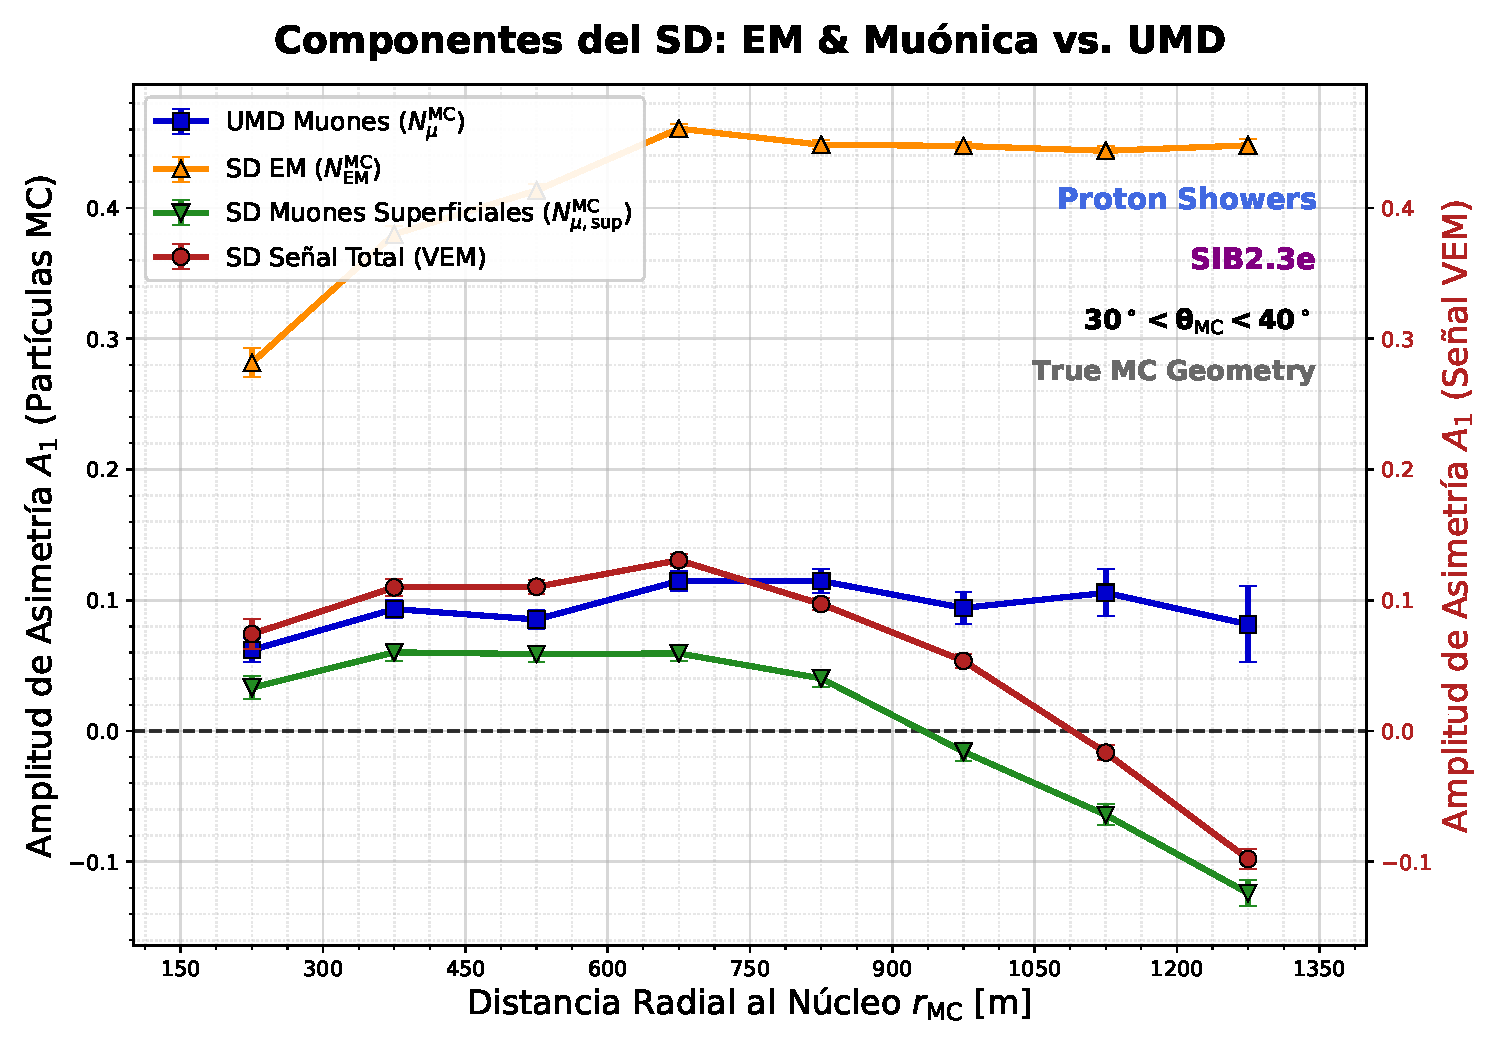
\includegraphics[width=\textwidth]{sd_desglose_componentes_vs_umd.pdf}
    \column{0.42\textwidth}
      \small
      \begin{tabular}{lccc}
        \toprule
        & $r{=}450$ & $r{=}800$ & $r{=}1200$~m\\
        \midrule
        \textcolor{itedaOrange}{\textbf{SD--EM}} & $+0.40$ & $+0.45$ & $+0.44$\\
        \textcolor{plotGreen}{\textbf{SD--$\mu$}} & $+0.05$ & $+0.04$ & \textbf{\textcolor{plotGreen}{$-0.10$}}\\
        \textcolor{plotMaroon}{\textbf{SD Total}} & $+0.11$ & $+0.09$ & \textbf{\textcolor{plotMaroon}{$-0.08$}}\\
        \textcolor{plotBlue}{\textbf{UMD $N_\mu$}} & $+0.10$ & $+0.12$ & $+0.11$\\
        \bottomrule
      \end{tabular}
      \vspace{0.4em}
      \begin{itemize}\small
        \item EM: fuertemente positiva en todo $r$ --- trazador puro de atenuación.
        \item Muones \emph{de superficie} (sin umbral): son los que invierten.
      \end{itemize}
  \end{columns}
\end{frame}

\begin{frame}{¿Qué explica la inversión del SD?}
  \vspace{1.4em}
  \centering
  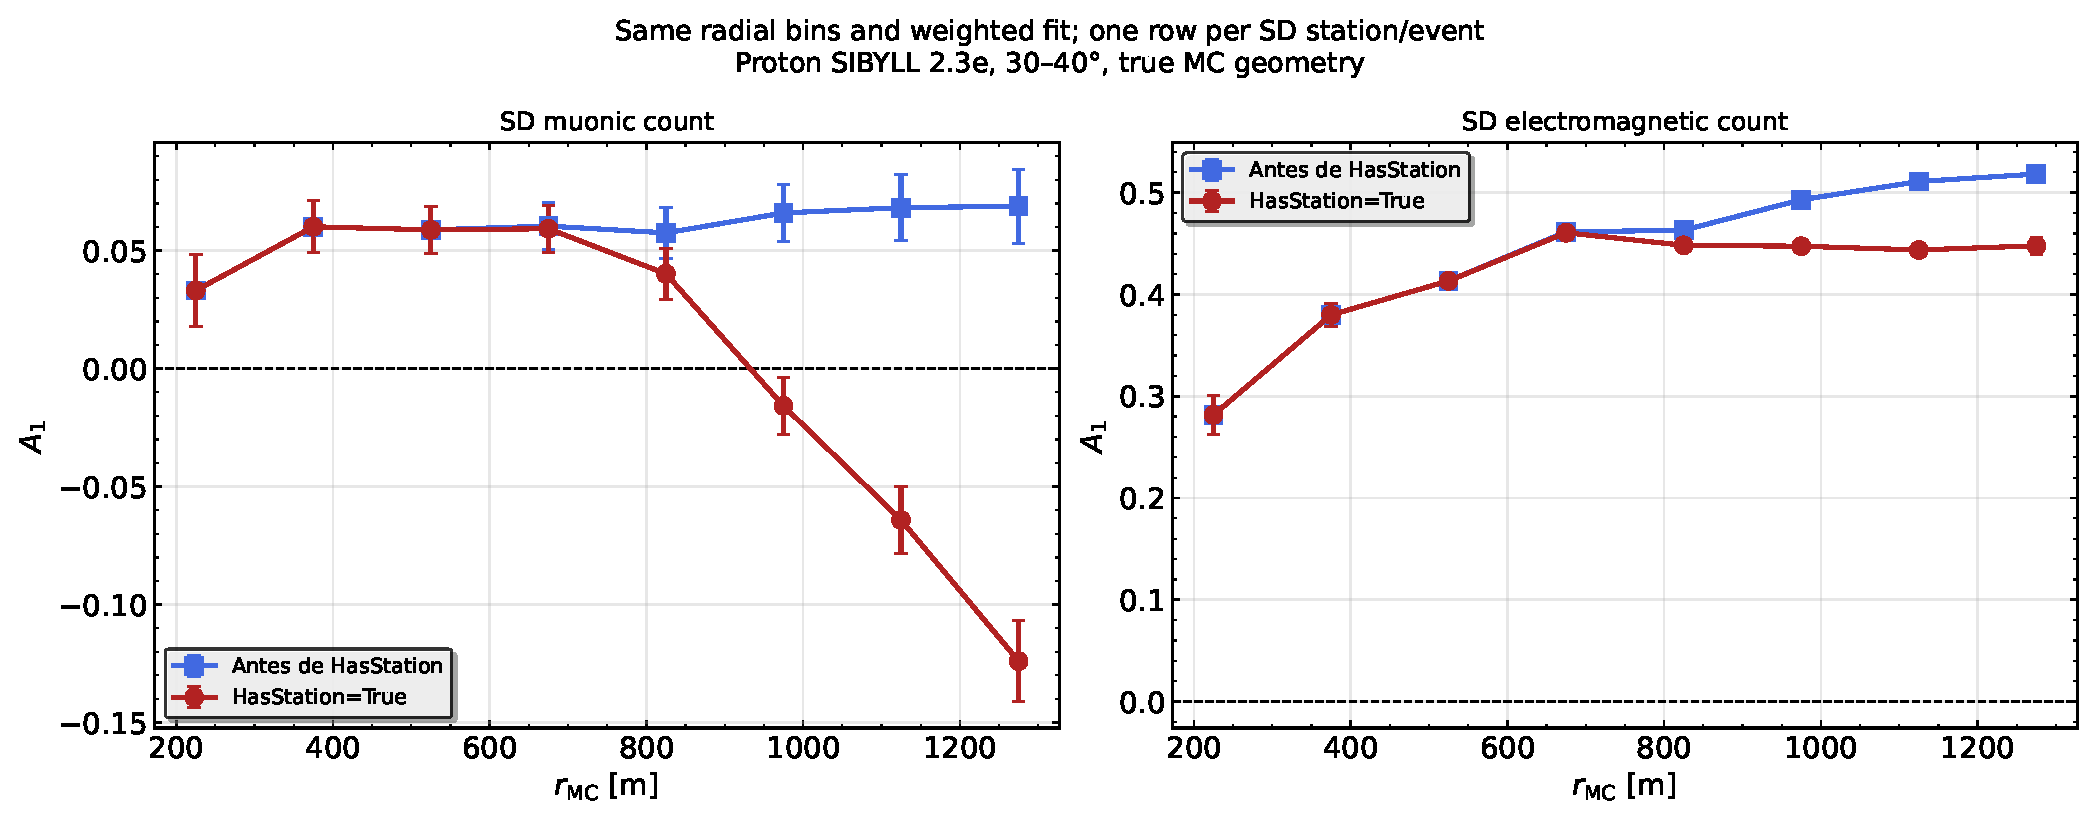
\includegraphics[width=0.78\textwidth,height=4.0cm,keepaspectratio]{sd_hasstation_antes_despues.pdf}
  \badgeCHECK

  \small
  \begin{itemize}
    \item Flag \texttt{HasStation} (umbral de reconstrucción del SD):
      \textbf{antes} de aplicarlo (azul) el conteo muónico se mantiene
      positivo, como el UMD; la EM (derecha) casi no cambia.
    \item \alert{Hipótesis en verificación}: el corte podría sesgar la
      muestra hacia eventos con componente muónica más dura.
  \end{itemize}
\end{frame}

% ============================================================
\section{Un segundo sistemático: el sesgo del núcleo}

\begin{frame}{Motivación}
  \badgeMC
  \begin{columns}[c]
    \column{0.42\textwidth}
      \textbf{Motivación}: ¿por qué $A_1^{REC}$ pierde magnitud respecto
      a $A_1^{MC}$?

      \vspace{0.8em}
      El residuo de conteo de muones tiene \textbf{media cercana a cero},
      pero su distribución no es simétrica: cola de sobre-reconstrucción,
      mayor en la región tardía.
    \column{0.5\textwidth}
      \centering
      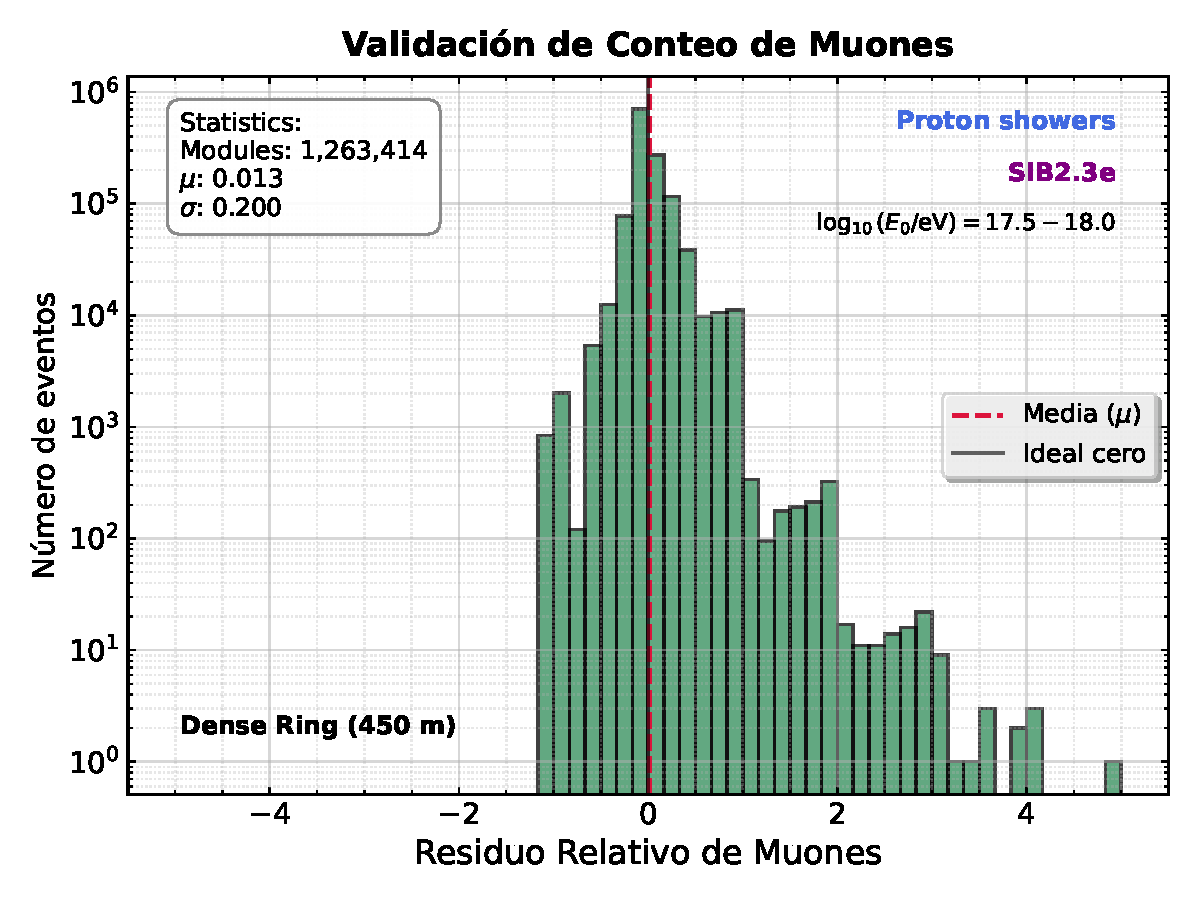
\includegraphics[width=\textwidth,height=5.4cm,keepaspectratio]{muon_counting_validation.pdf}
  \end{columns}
\end{frame}

\begin{frame}{El núcleo reconstruido se corre a lo largo del eje temprano-tardío}
  \badgeMC
  \vspace{-0.6em}
  \begin{columns}[T]
    \column{0.55\textwidth}
      \centering
      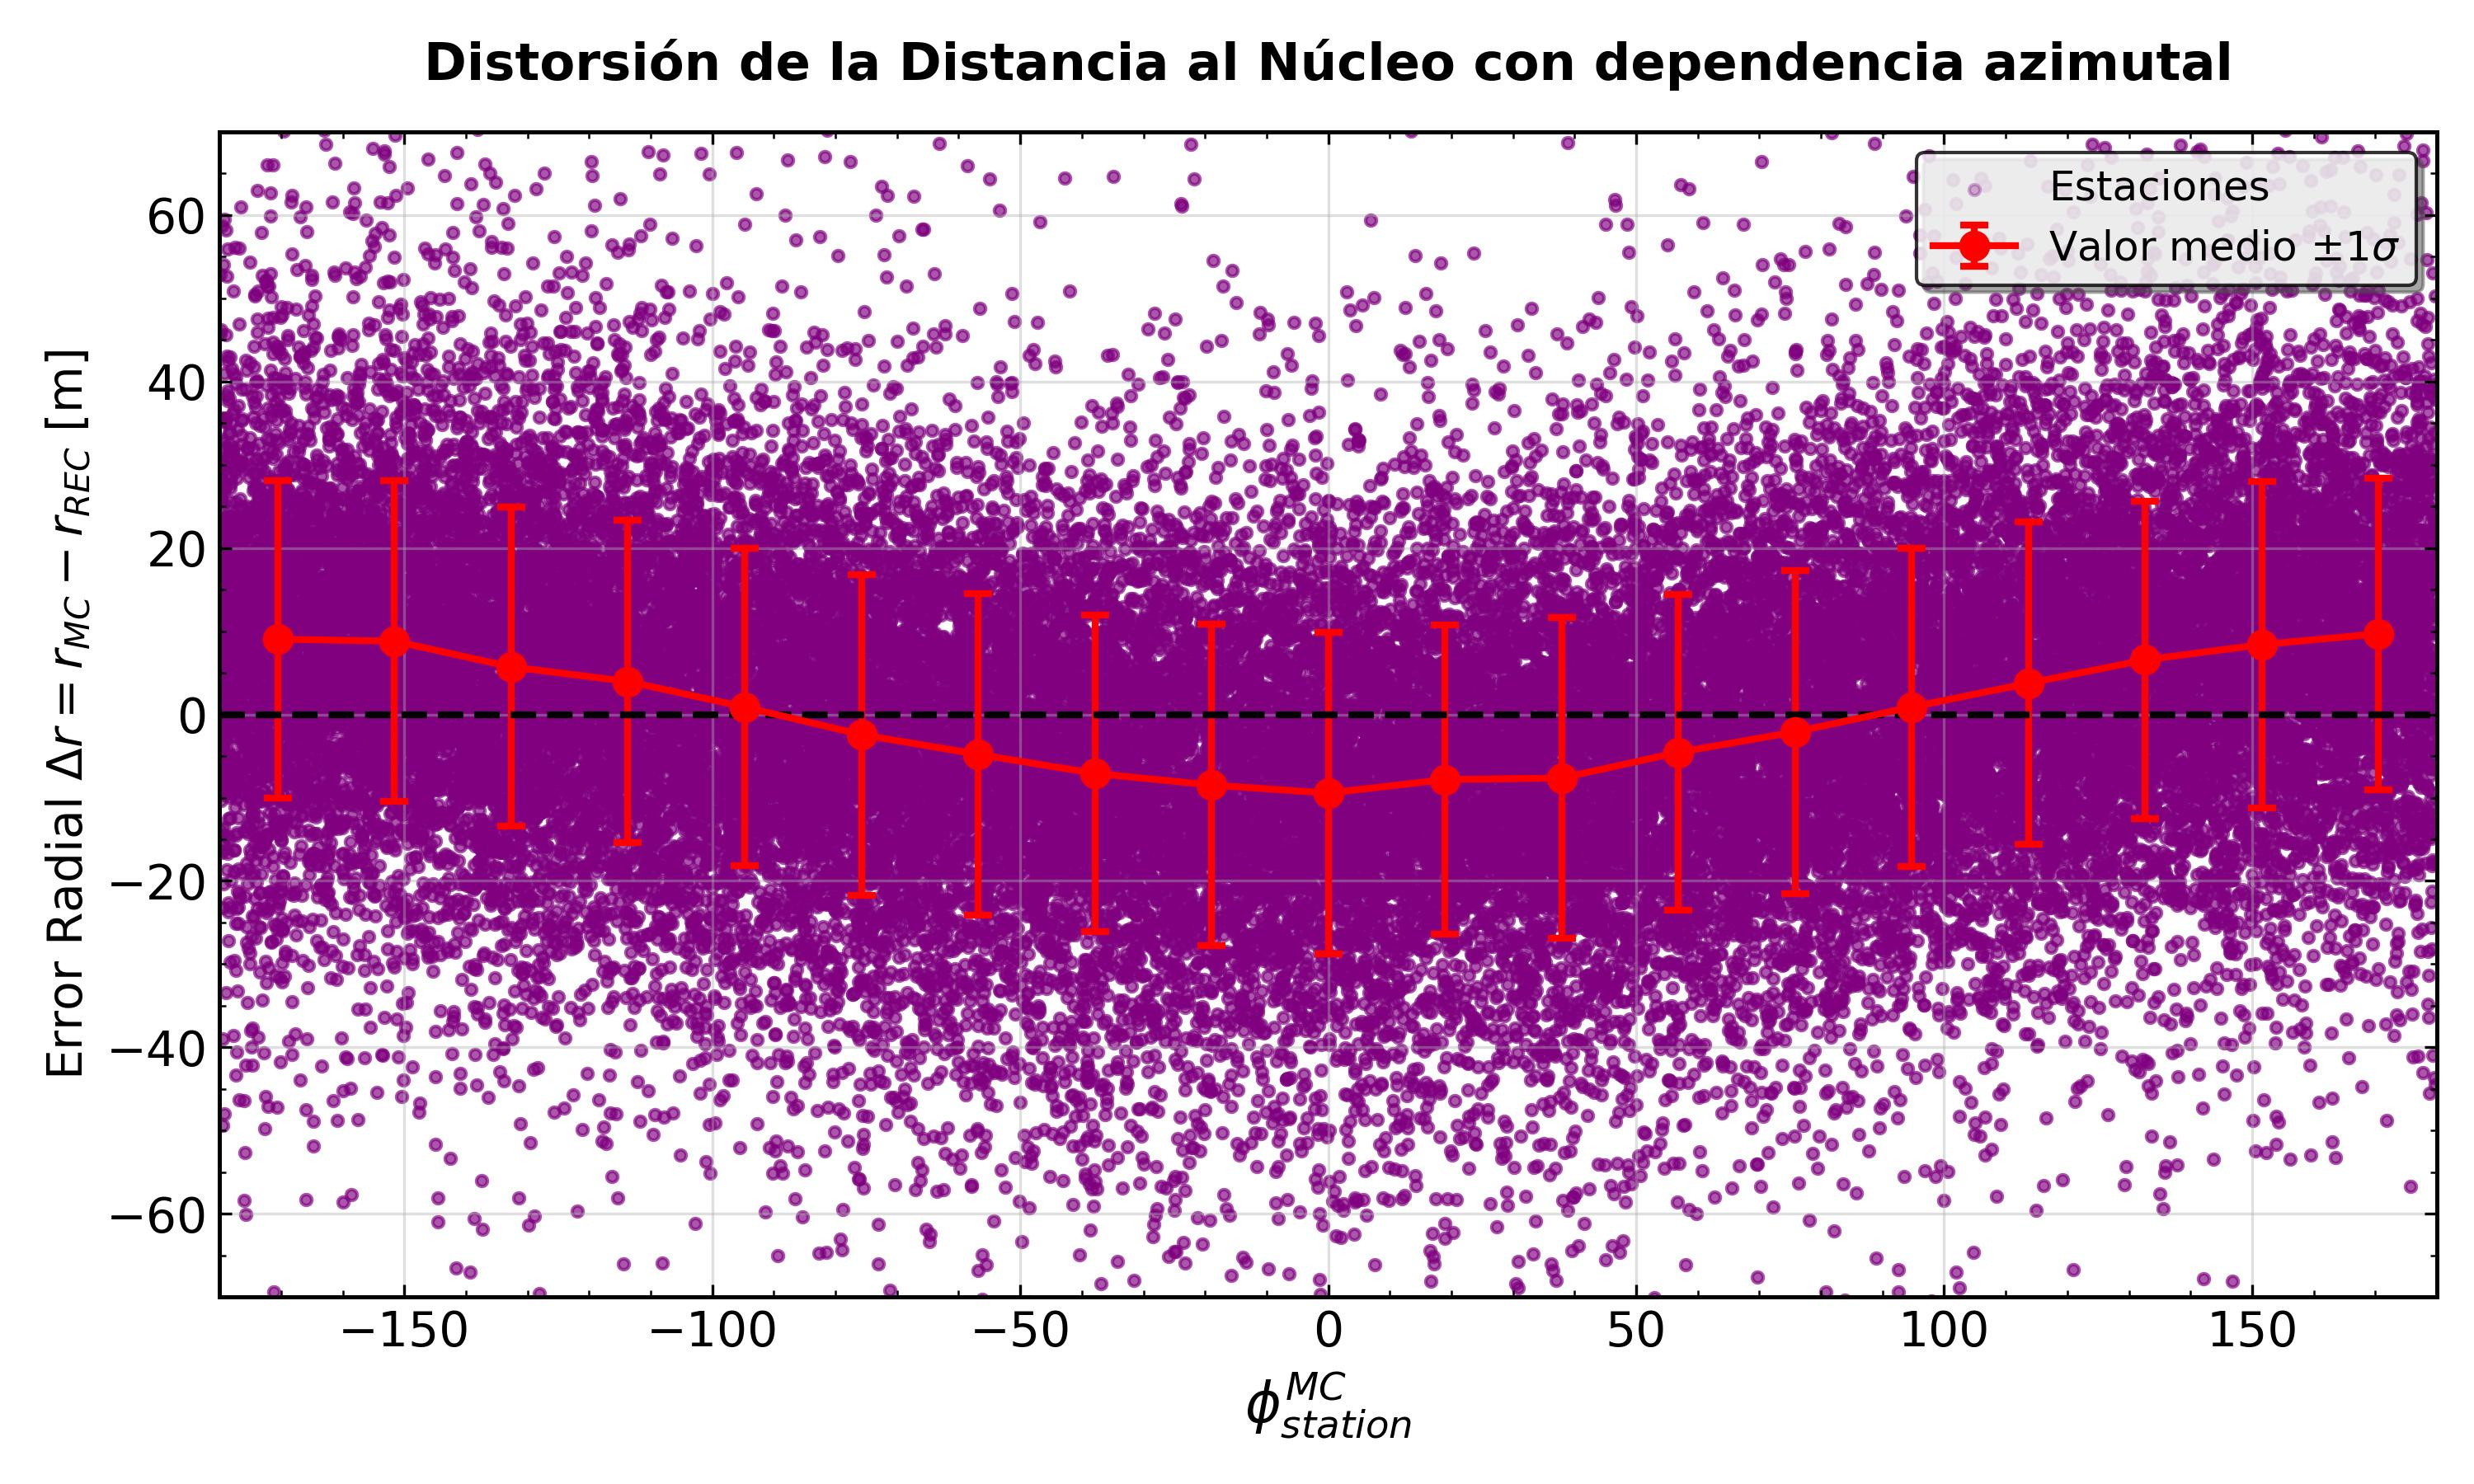
\includegraphics[width=\textwidth,height=5.1cm,keepaspectratio]{error_radial_azimut.jpg}
    \column{0.4\textwidth}
      \begin{itemize}\small
        \item \textbf{Error en la posición del núcleo} reconstruido
          respecto a la posición real de Monte Carlo
          ($\Delta r = r_{MC}-r_{REC}$), vs.\ $\phi_{MC}$ de la estación.
        \item Región temprana ($\phi\approx0^\circ$): $\Delta r<0$ ---
          el núcleo queda \textbf{más lejos}.
        \item Región tardía ($\phi\approx\pm180^\circ$): $\Delta r>0$ ---
          queda \textbf{más cerca}.
      \end{itemize}
  \end{columns}
  \vspace{-0.6em}
  \begin{center}
  \small\alert{Este alineamiento sistemático del sesgo de reconstrucción
  con el eje temprano-tardío es uno de los resultados centrales de este
  análisis.}
  \end{center}
\end{frame}

\begin{frame}{Por qué: una LDF simétrica ajustada a una señal asimétrica}
  \badgeMC
  \begin{columns}[c]
    \column{0.44\textwidth}
      \begin{itemize}\small
        \item \textit{Offline} ajusta la LDF asumiéndola \textbf{simétrica
          en $\phi$}; el único grado de libertad para absorber el
          exceso/déficit real es la \textbf{posición del núcleo}.
      \end{itemize}
    \column{0.5\textwidth}
      \centering
      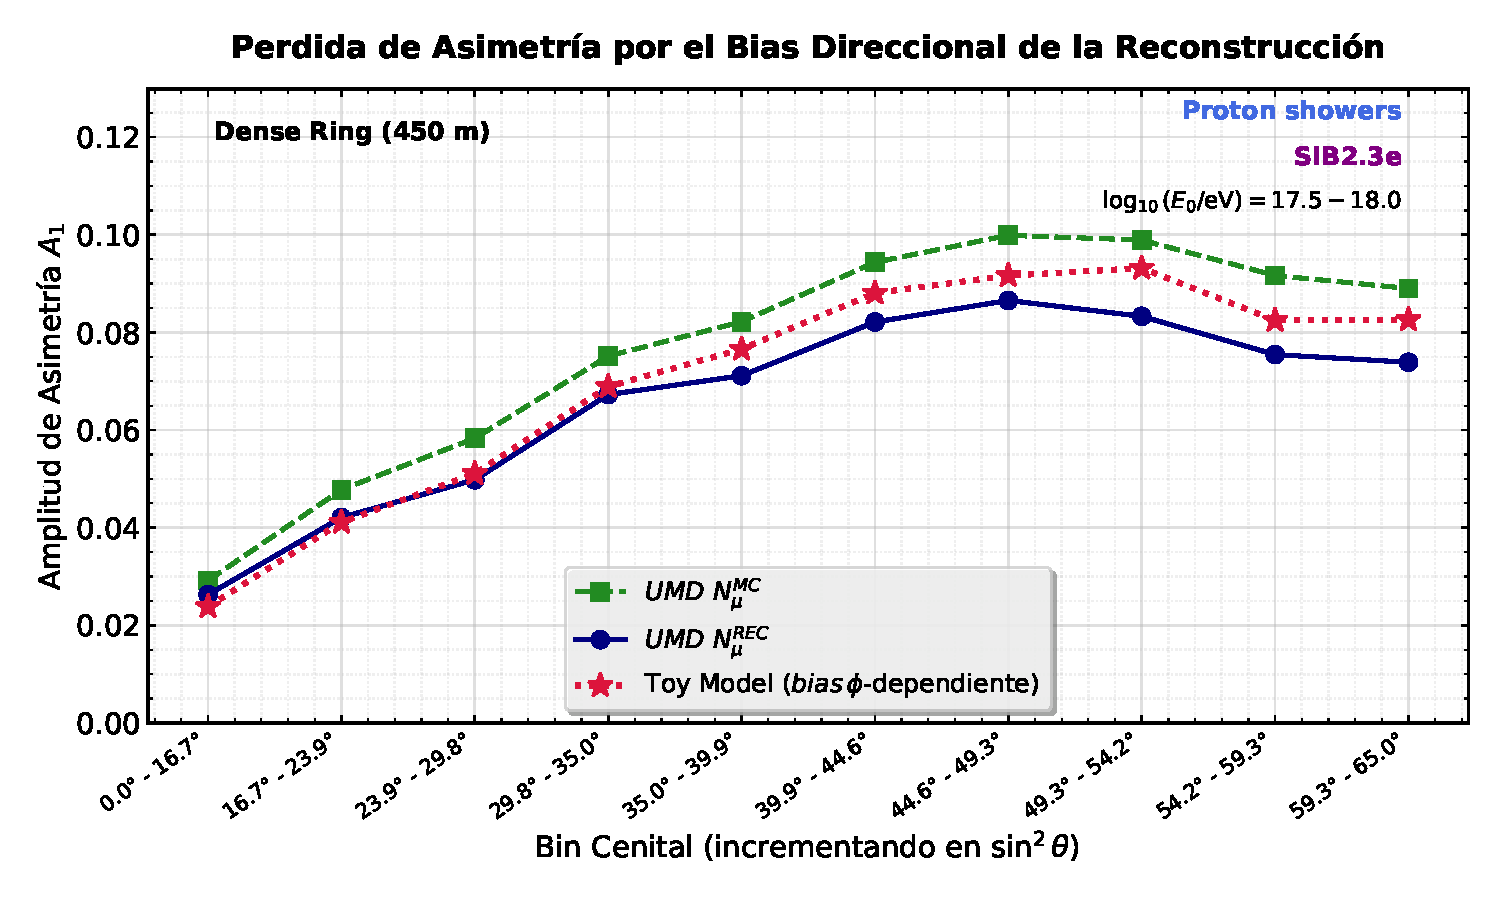
\includegraphics[width=\textwidth,height=4.8cm,keepaspectratio]{toy_model.pdf}
  \end{columns}
  \small \emph{Toy Model} (\emph{bootstrap} sobre ese residuo, inyectado
  sobre $N_\mu^{MC}$): reproduce \textbf{exactamente} la caída de $A_1$
  para $\theta\lesssim35^\circ$; explica $>50\%$ para $\theta\gtrsim35^\circ$.
\end{frame}

% ============================================================
\section{Hacia los datos reales}

\begin{frame}{Primera señal en datos reales del \textit{Infill}}
  \badgeDATA
  \begin{columns}[c]
    \column{0.58\textwidth}
      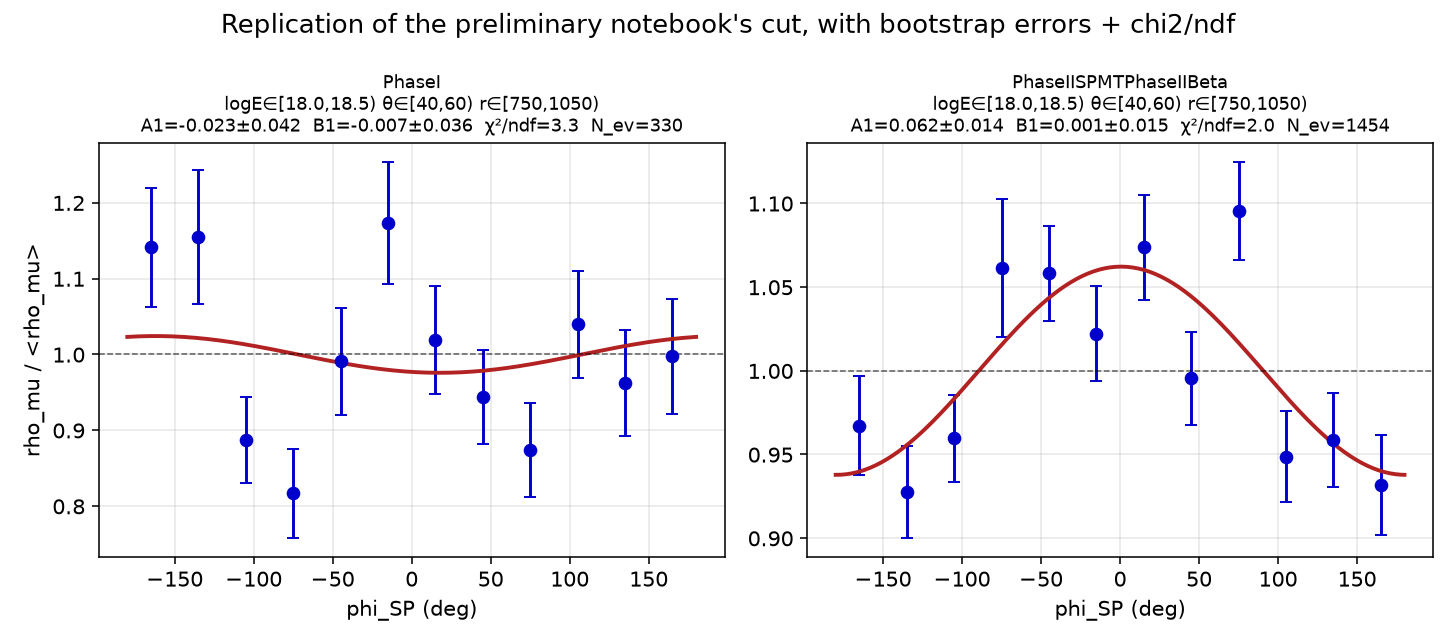
\includegraphics[width=\textwidth]{datos_reales_replicacion.png}
    \column{0.38\textwidth}
      \begin{itemize}
        \item $\log_{10}(E/\text{eV})\in[17.5,18.0)$, $\theta\in[50^\circ,65^\circ)$,
          $r\in[750,900)$~m.
        \item \alert{$A_1=+0.067\pm0.014$}, $\chi^2/\text{ndf}=2.3$,
          6193 eventos, \textbf{4.8$\sigma$}.
        \item Signo correcto, magnitud consistente con las simulaciones.
        \item \emph{Resultados preliminares} con datos reales de Auger ---
          pipeline de datos de campo ya operativo.
      \end{itemize}
  \end{columns}
\end{frame}

% ============================================================
\section{Conclusiones y próximos pasos}

\begin{frame}{Conclusiones}
  \begin{enumerate}
    \item El UMD aísla, por primera vez, la asimetría azimutal de una señal
      \textbf{puramente muónica} --- y esa asimetría es medible, robusta y
      un \textbf{discriminador de masa} viable ($MF\approx2.5$).
    \item El contraste UMD/SD revela una \textbf{inversión de signo del SD}
      real y no trivial --- explicada del lado del UMD, todavía
      \textbf{abierta} del lado del SD.
    \item Los primeros datos reales del \textit{Infill} muestran una señal
      \textbf{positiva y significativa} ($4.8\sigma$), con un sistemático de
      exposición angular identificado y en corrección.
  \end{enumerate}
  \vspace{0.5em}
  \begin{block}{Próximos pasos}
    Barrido completo del espacio de parámetros (energía, $\theta$, $r$) en
    datos reales de Auger, y cierre del estudio de la inversión del SD.
  \end{block}
\end{frame}

\begin{frame}[standout]
  ¡Gracias!\\[0.4em]
  \small lautarosilvapizzi@gmail.com
\end{frame}

% ============================================================
\appendix

\begin{frame}{Backup: bondad de ajuste UMD vs.\ SD}
  \badgeMC
  \centering
  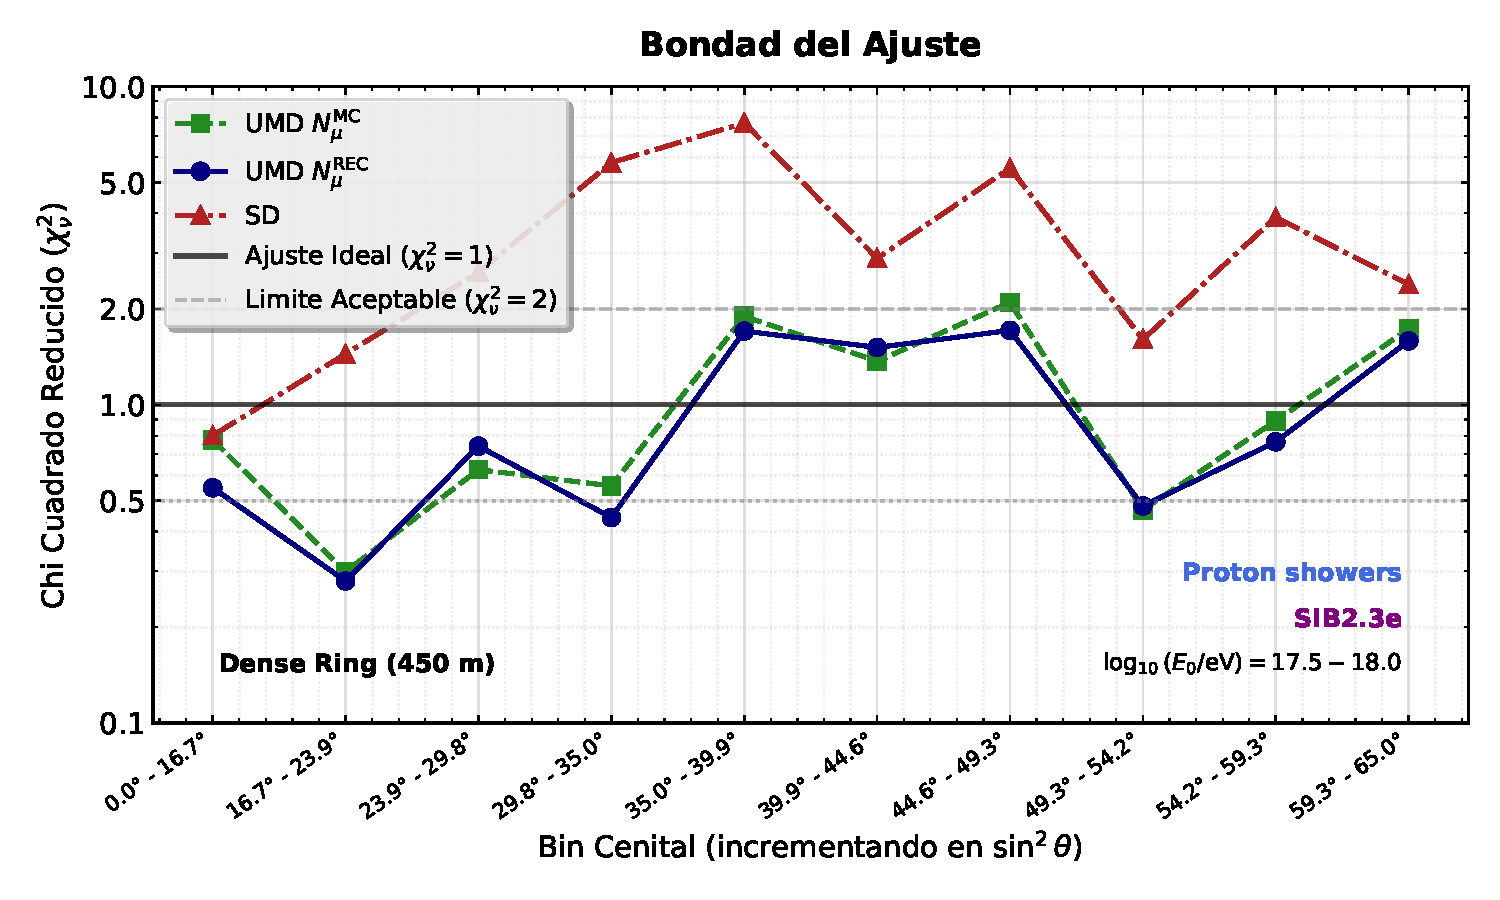
\includegraphics[width=0.6\textwidth,height=4.4cm,keepaspectratio]{chi2_reduced_fits.pdf}
  \begin{itemize}\small
    \item UMD (MC y REC): $\chi^2_\nu\approx1$ en todo el rango.
    \item SD: hasta $\chi^2_\nu\sim10$ --- no es una falla del modelo, sino la
      enorme estadística EM haciendo visibles desviaciones de segundo orden.
  \end{itemize}
\end{frame}

\begin{frame}{Backup: el sesgo de conteo direccional que alimenta el \emph{Toy Model}}
  \badgeMC
  \centering
  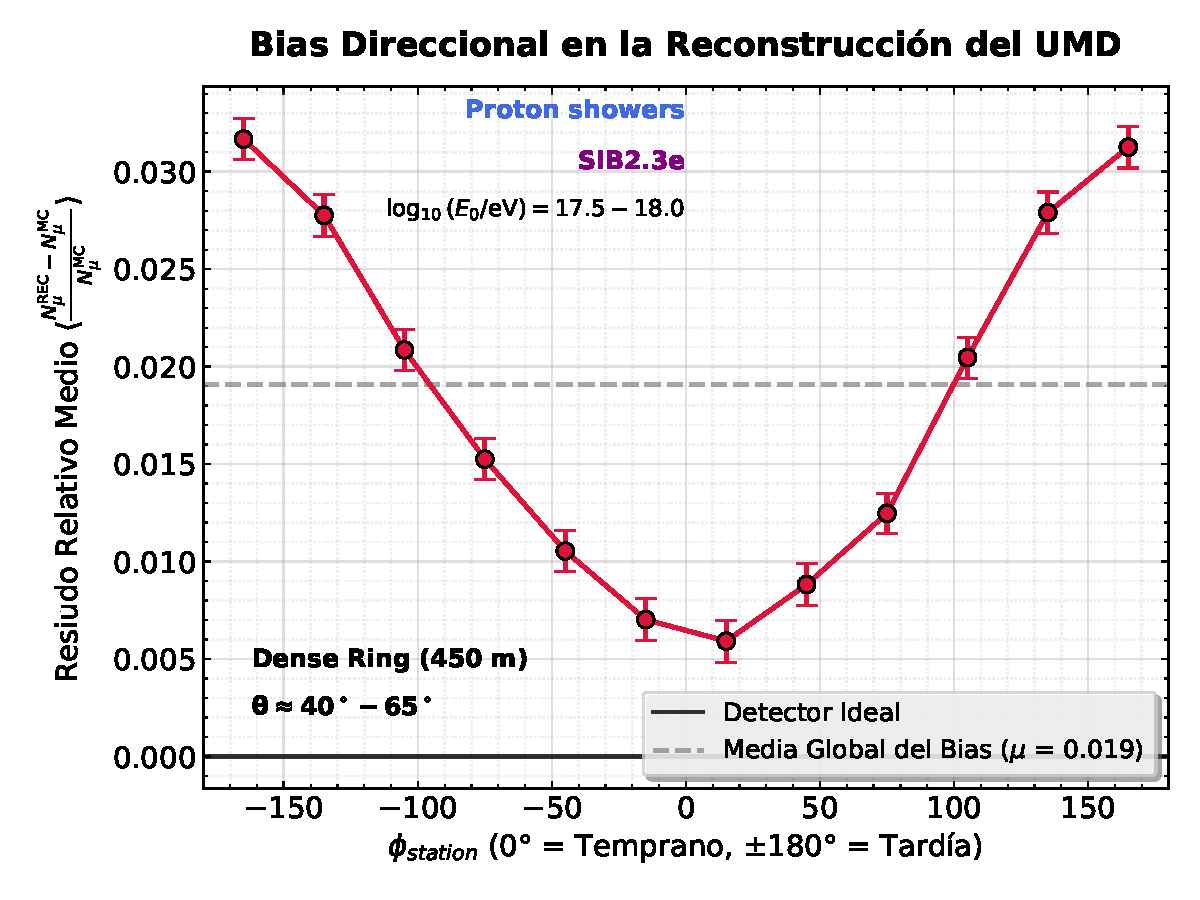
\includegraphics[width=0.55\textwidth,height=4.3cm,keepaspectratio]{directional_bias.pdf}

  \vspace{0.5em}
  \small El residuo relativo de reconstrucción de muones es sistemáticamente
  mayor en la región tardía (baja densidad) que en la temprana --- este
  residuo, segmentado por $\phi$, es lo que se inyecta en el \emph{Toy Model}.
\end{frame}

\begin{frame}{Backup: el sistemático de exposición angular en datos reales}
  \badgeDATA
  \begin{columns}[T]
    \column{0.6\textwidth}
      \centering
      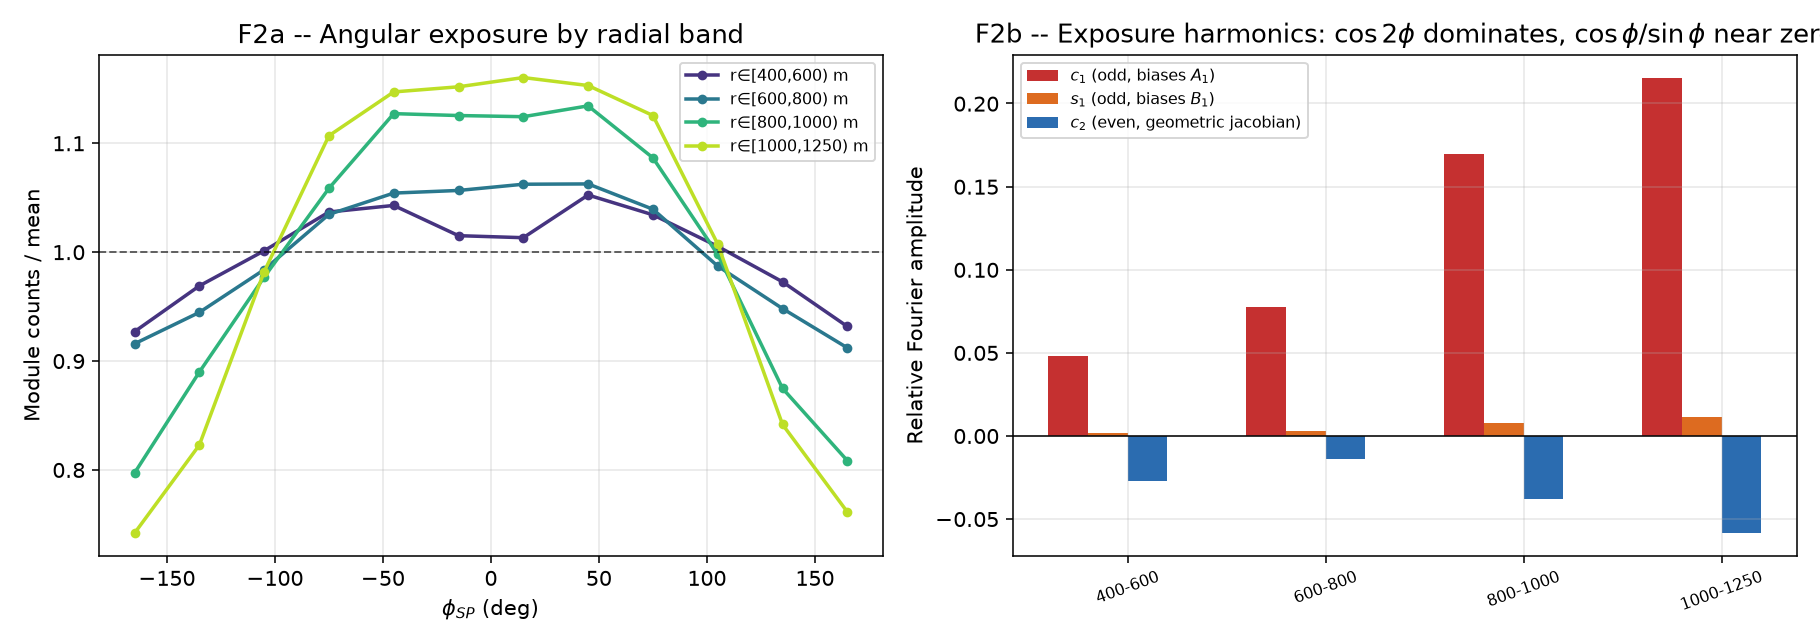
\includegraphics[width=\textwidth,height=4.1cm,keepaspectratio]{datos_reales_exposicion_phi.png}
    \column{0.36\textwidth}
      \begin{itemize}\small
        \item La geometría real del \emph{Infill} no expone las 12 fases
          $\phi_{SP}$ por igual.
        \item El término $\cos\phi$ de esa exposición ---el mismo armónico
          que se ajusta--- crece con $r$: $0.05\to0.22$ de 450 a 1200~m.
        \item A $r\gtrsim1$~km es \textbf{comparable} a $A_1$ del Anillo Denso.
      \end{itemize}
  \end{columns}
  \vspace{0.1em}
  \small \alert{Próximo paso}: corregir por exposición antes de reportar $A_1$
  como medición de composición.
\end{frame}

\begin{frame}{Backup: galería de ajustes \textit{Infill}, ejemplo $30^\circ$--$40^\circ$}
  \badgeMC
  \begin{columns}[T]
    \column{0.5\textwidth}
      \centering\footnotesize Geometría Monte Carlo\\
      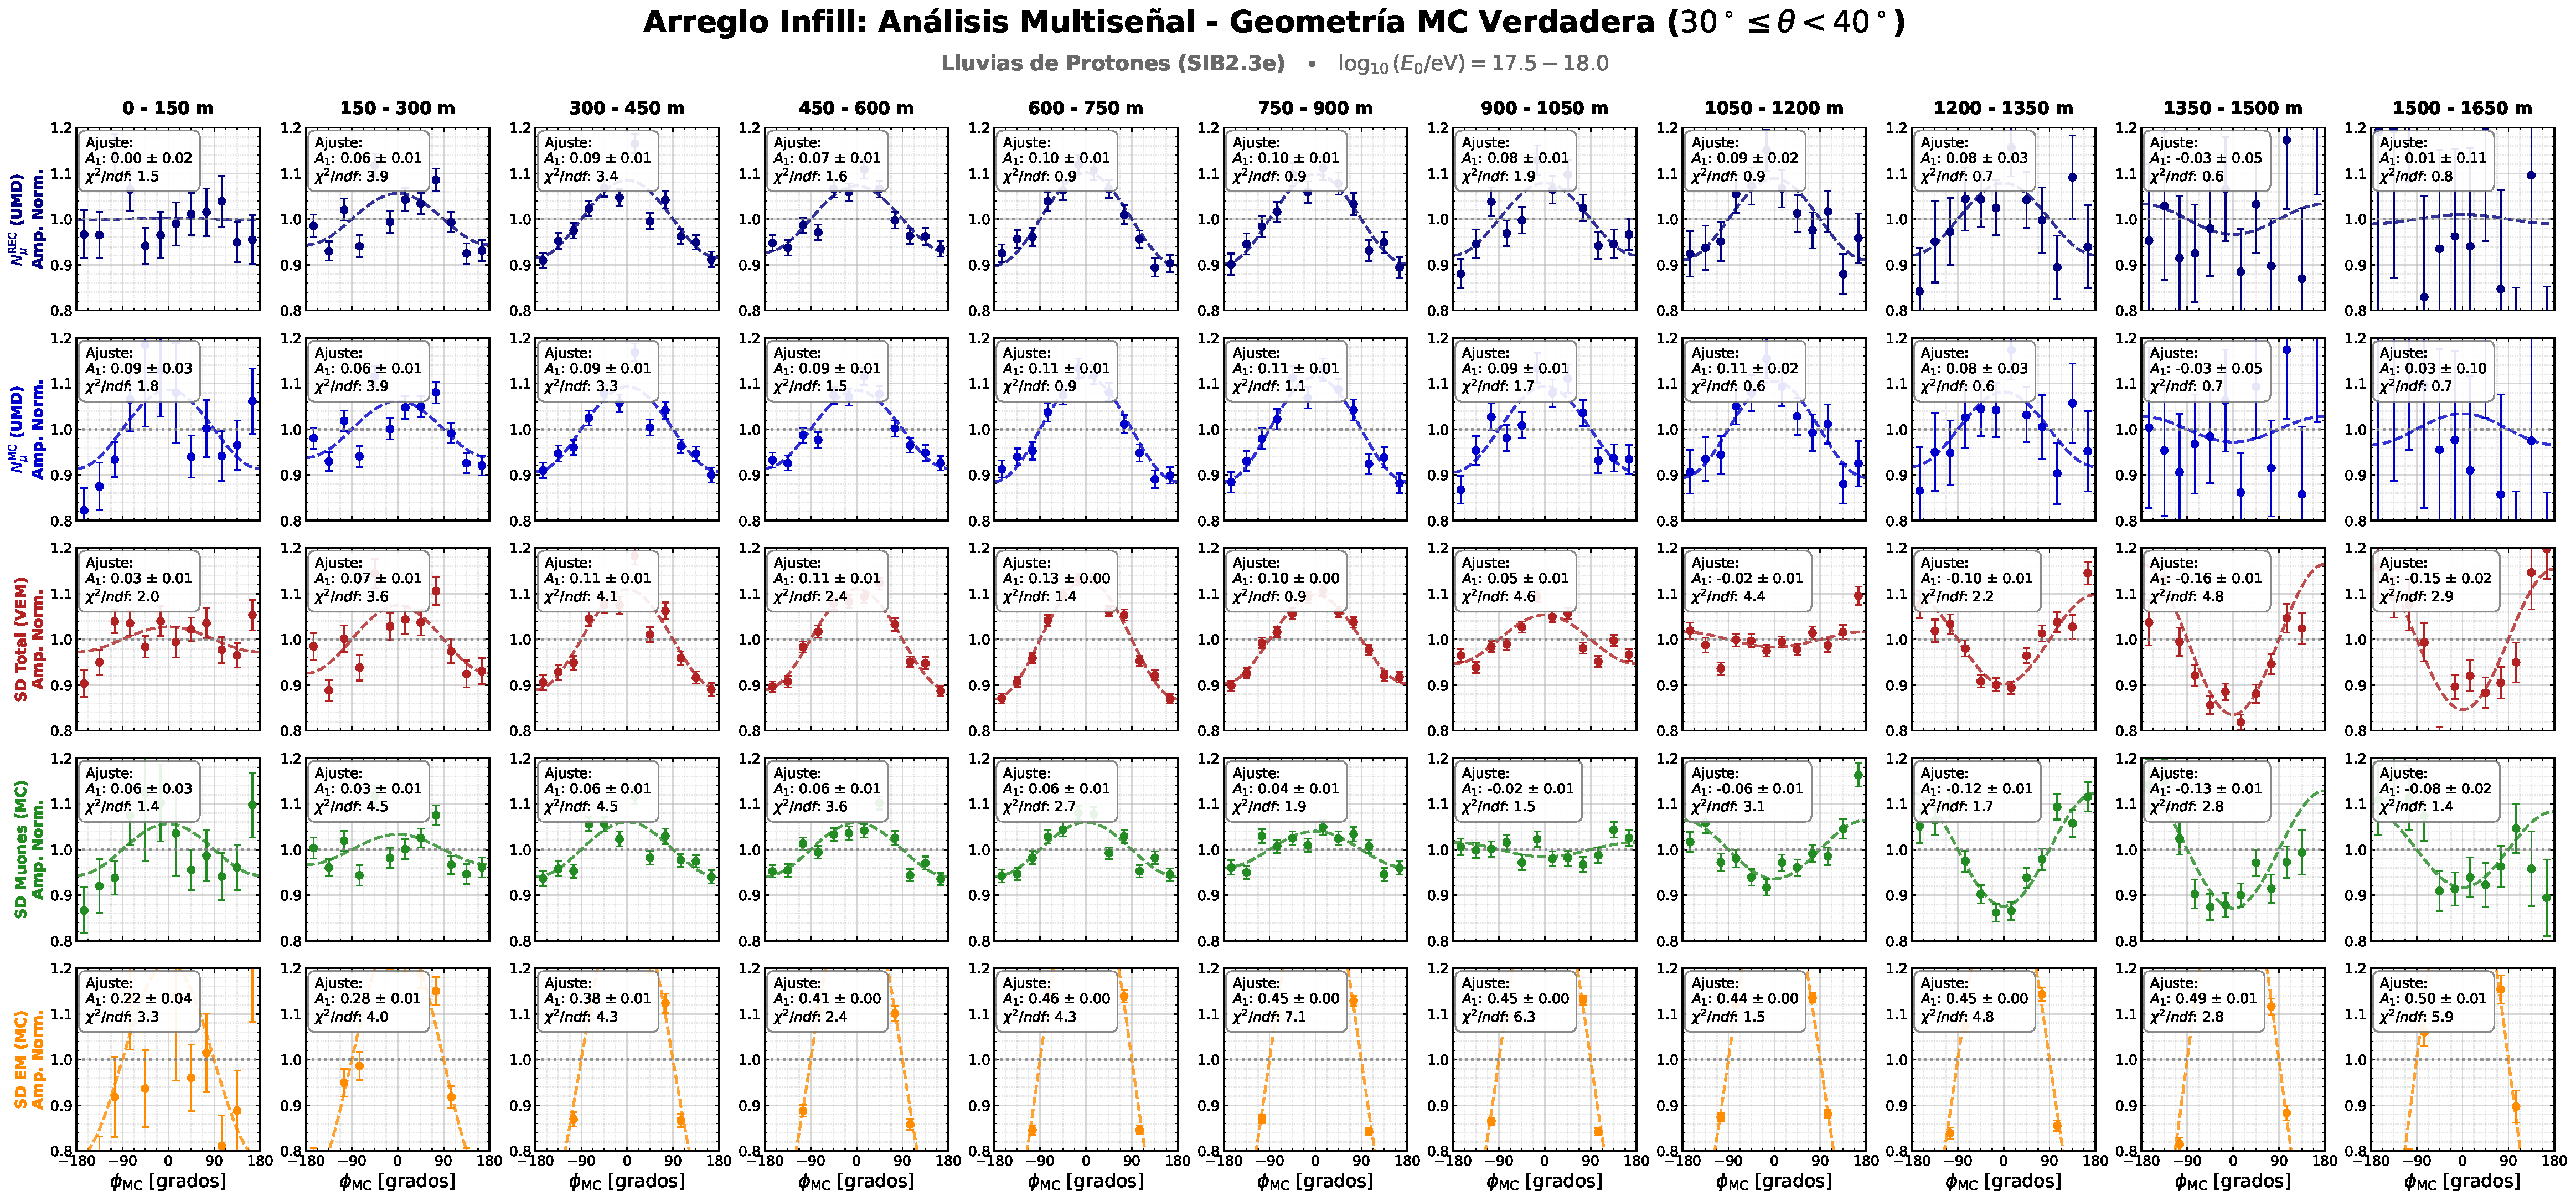
\includegraphics[width=\textwidth]{anexo_grilla_mc_30_40.pdf}
    \column{0.5\textwidth}
      \centering\footnotesize Geometría reconstruida\\
      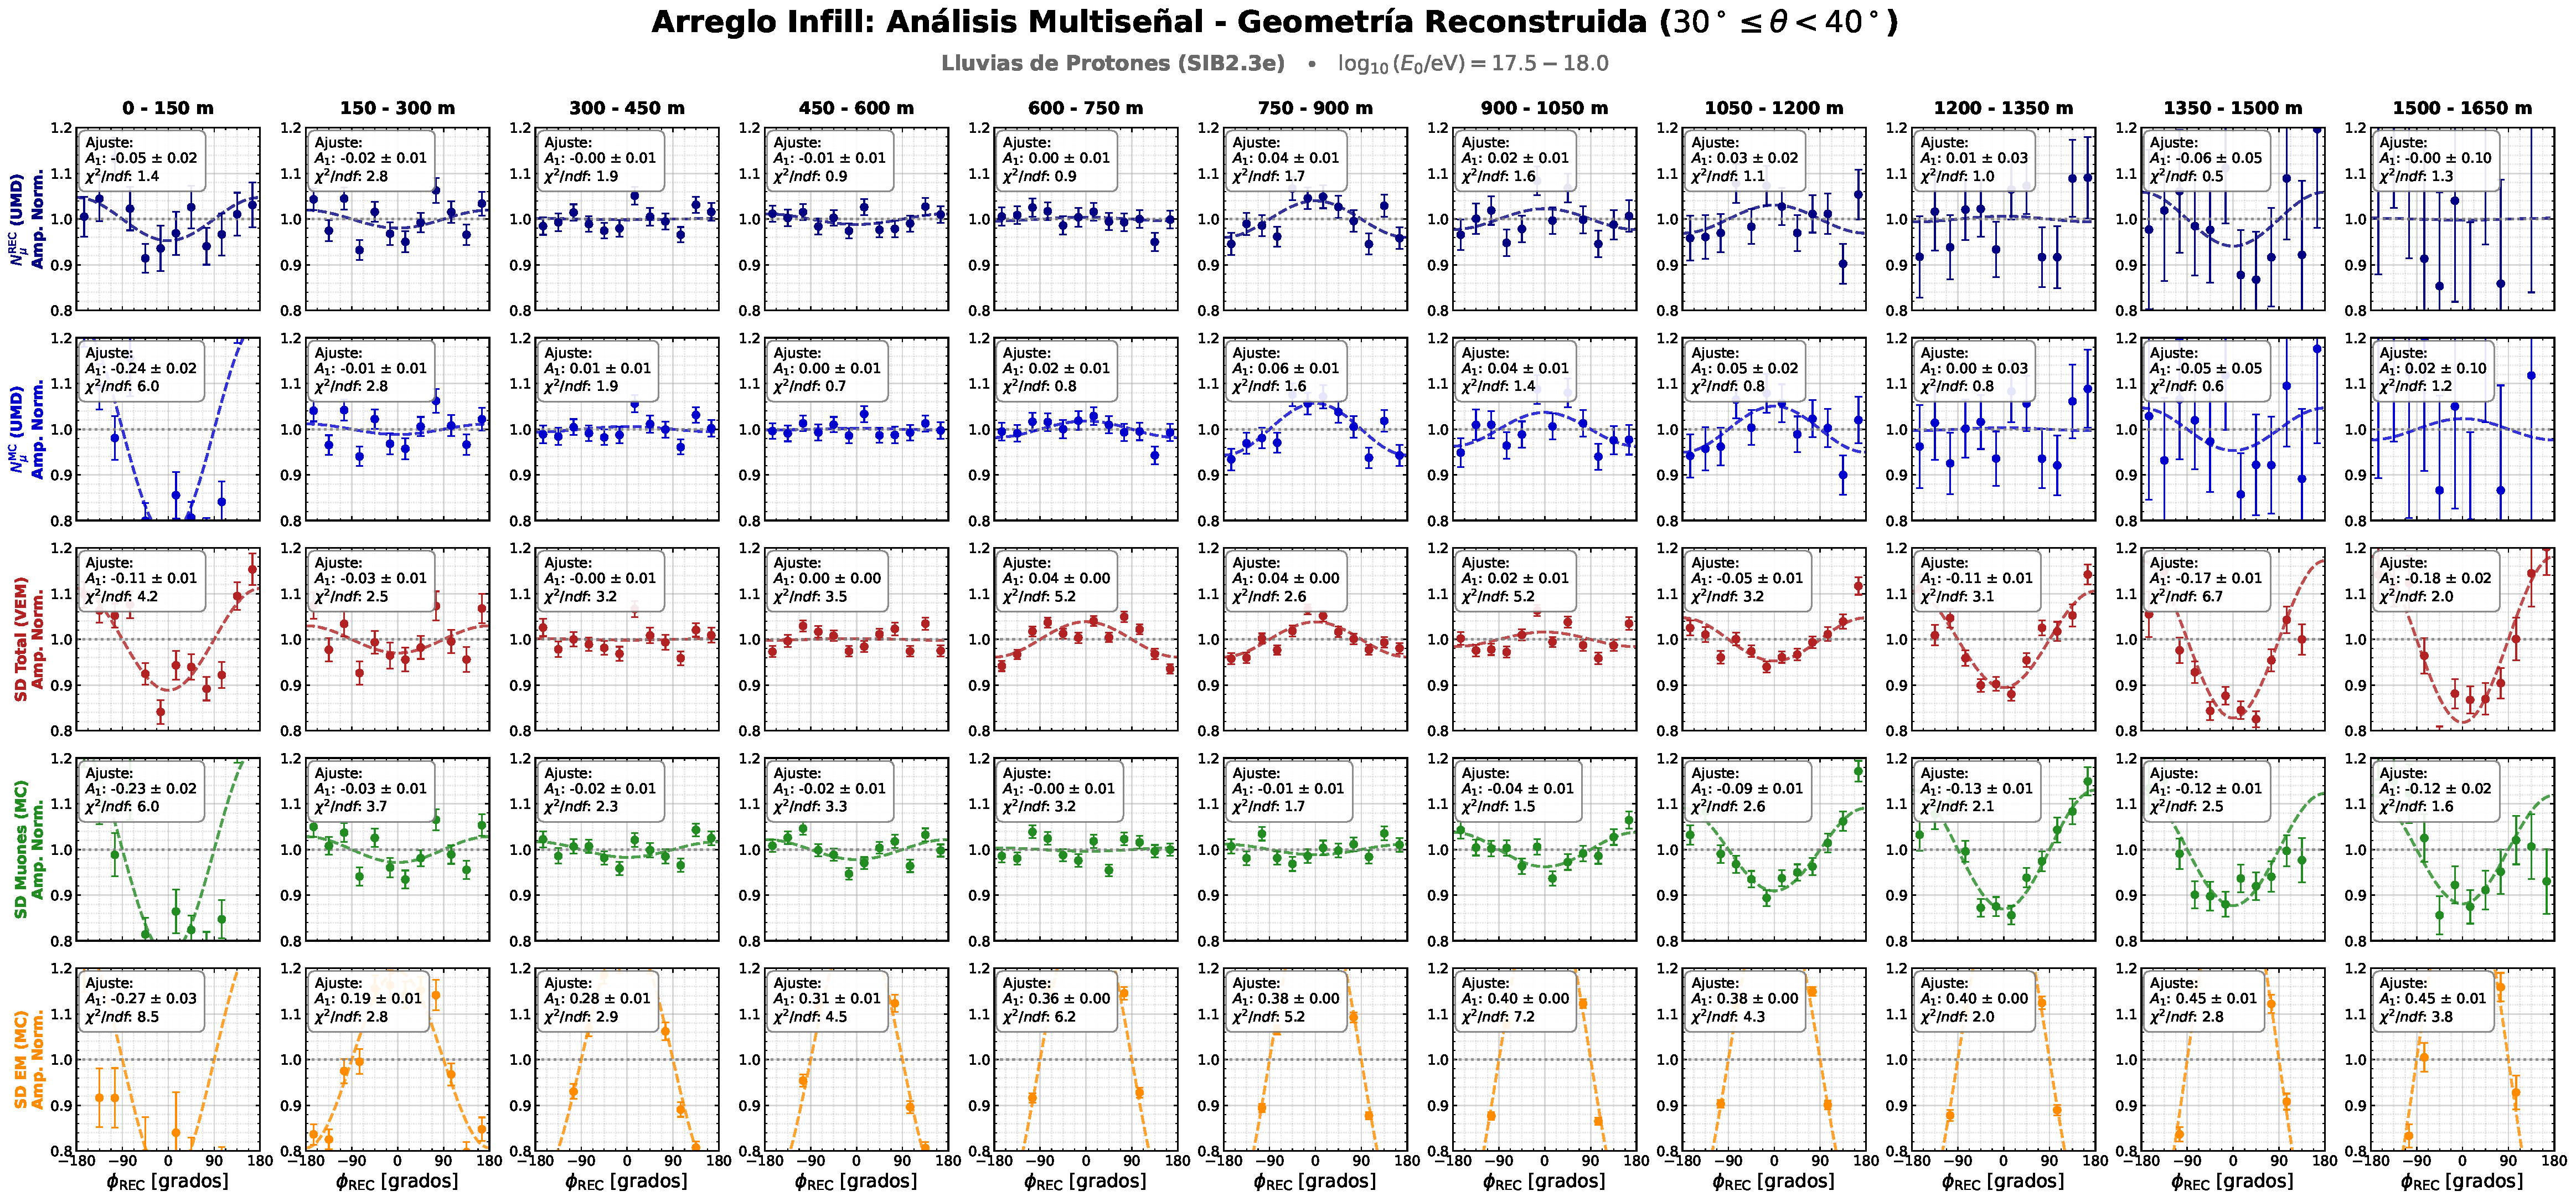
\includegraphics[width=\textwidth]{anexo_grilla_rec_30_40.pdf}
  \end{columns}
\end{frame}

\end{document}
